\documentclass[runningheads]{llncs}
%
\usepackage{graphicx}

\usepackage{natbib}
\setcitestyle{square,numbers}

\usepackage[toc,page]{appendix}

\usepackage{nameref}

% \usepackage{amsthm}
\usepackage{amsmath}
\usepackage{amssymb}
\usepackage[ruled,vlined]{algorithm2e}

\usepackage{xcolor}
\usepackage{color,soul}
\usepackage{pdfpages}

\def\HiLi{\leavevmode\rlap{\hbox to \hsize{\color{yellow!50}\leaders\hrule height .8\baselineskip depth .5ex\hfill}}}
         
\newcount\Comments  % 0 suppresses notes to selves in text
\Comments=0
\definecolor{darkgreen}{rgb}{0,0.6,0}         
         
\newcommand{\kibitz}[2]{\ifnum\Comments=1{\color{#1}{#2}}\fi}
\newcommand{\rmr}[1]{\kibitz{red}{[Reshef says:#1]}}
\newcommand{\rf}[1]{\kibitz{blue}{[Roy says:#1]}}
\newcommand{\kg}[1]{\kibitz{darkgreen}{[Kobi says:#1]}}

\begin{document}

%
\title{Proportional Participatory Budgeting with Substitute Projects}
%
%\titlerunning{Abbreviated paper title}
% If the paper title is too long for the running head, you can set
% an abbreviated paper title here
%

\author{Anonymous Submission X}
% \author{Roy Fairstein\inst{1} \and
% Reshef Meir\inst{2} \and
% Kobi Gal\inst{1,3}}
% \author{Roy Fairstein\inst{1}\orcidID{0000-0002-2352-5200} \and
% Reshef Meir\inst{2}\orcidID{0000-0003-0961-3965} \and
% Kobi Gal\inst{1,3}\orcidID{0000-0001-7187-8572}}
%
\authorrunning{Submission X}
% \institute{}
% \authorrunning{Fairstein et al.}
% First names are abbreviated in the running head.
% If there are more than two authors, 'et al.' is used.
%
% \institute{Ben-Gurion Univ. of the Negev, Israel \and
% Technion, Israel Institute of Technology \and
% University of Edinburgh, U.K.}
%
\maketitle              % typeset the header of the contribution
%
\begin{abstract}
Participatory budgeting is a democratic process for allocating funds to projects based on the votes of members of the community.  However, most input methods of voters' preferences  prevent the voters from expressing 
complex relationships among projects, 
 leading to outcomes that do not reflect their preferences well enough. In this paper, we propose an  input method that begins to address this challenge, by  allowing  participants to express substitutes over projects.  Then, we extend a known aggregation mechanism    from the literature (Rule~X) to handle substitute projects. We  prove that our extended rule preserves proportionality under natural conditions, and show empirically that it obtains  substantially more welfare than the original mechanism on instances with substitutes.

\keywords{Participatory Budgeting, Social Choice, Fairness}
\end{abstract}
%
%
%
\section{Introduction}

%The first Participatory budgeting project had started a while back in Brazil in the 1980s \cite{cabannes2004participatory}, with the goal of creating a more transparent funding process and giving more power to citizens. Since then, 
Participatory budgeting (PB) is gaining increased attention from both researchers and practitioners  and is actively in use in  cities around the world~\cite{su2017porto}. 
% world~\cite{pape2016budgeting, su2017porto, sintomer2008porto}. 
%In participatory budgeting  citizens decide how to allocate some common budget in order to fund projects that will increase their life quality. The 
This process typically includes several steps. In the first step,  citizens suggest and discuss  different projects, resulting with a   list of feasible projects and  their cost estimation. Next,  citizens vote on which of the projects they would like to  fund. Finally, the votes are aggregated by a mechanism that selects a subset of projects to fund.
Different  input formats exist that allow  voters to express their preferences over    projects, such as approval voting, knapsack ranking and additive utility (specified later on). %\cite{aziz2021participatory,goel2019knapsack, benade2020preference,peters2020proportional}. 
% \cite{aziz2021participatory,goel2016knapsack,aziz2020expanding, benade2020preference,peters2020proportional}. 


In the real world, voters' preferences may exhibit complex relationships between projects. For example,  the utility from one project might depend on whether some other project is funded or not \cite{jain2020participatory, jain2021partition}.
Consider for example a city where there are 4 different suggestions to build a large parking lot in different places, as well as two unrelated projects (say, a playground and a library). The budget is sufficient for only four projects.
There is a severe parking problem, so most citizens will assign higher utility to parking lots than to the other projects (or rank parking lots higher than other projects). As a result all 4 parking lots are likely to be funded and consume the entire budget, even if one or two parking lots are sufficient to solve most of the parking shortage.
A better outcome that leads to a higher social welfare would have been to fund only two parking lots, and in addition the playground and the library. 

The above problem occurs since common mechanisms   ignore the fact that the four parking lots are \emph{substitutes}.   The existence of substitutes raises multiple challenges, from how to represent utilities efficiently, via simple elicitation, and eventually how to modify voting rules to take them into account.
%Indeed, additive cardinal utilities or rankings cannot convey such relations. 

\paragraph{Our contribution} 
%We extend an aggregation mechanism  called Rule X \cite{peters2020proportional} to handle substitute projects (SRX) and analyze it both theoretically and empirically.
We first extend the input format suggested by \citet{jain2020participatory} for substitute projects. Then, we modify the iterative Rule~X (RX) to a mechanism~\cite{peters2020proportionality} called Substitute Rule~X (SRX) by updating the utility of the projects for each voter according to their reported marginal utility functions.


On the theory side,  we define a weakened version of proportionality notion from the literature to fit the case of substitutes, and prove SRX preserves proportionality under natural conditions. 

We also show empirically that SRX obtains substantially higher welfare than RX on instances with substitutes while maintaining a fair allocation.

% Our contribution can be summarised by: \rmr{add paragraph title}
% \begin{enumerate}
%     \item Generalizing \cite{jain2020participatory} input format for individual partitions. 
%     \item A natural extension to RX in order to handle votes with substitutes called SRX.
%     \item Proving SRX holds two notions of proportionality under natural conditions.
%     \item Extensive simulations which shows improved welfare compared to the original RX.
% \end{enumerate}
% \rmr{I don't understand why you describe contribution twice: without bullets and then with bullets}\rf{wasn't sure about it, can remove the bullets completely. added it just to have a paragraph with contribution title}\rmr{decide if you want bullets or not. if yes - list all contributions (only) there. if not - make sure you write everything without bullets.}

% \rf{solution to the problem}In this paper,  we suggest an input format and aggregation mechanism which allow  voters to express substitute relationships and output socially beneficial outcomes.
%  Our input format  allows  the voters to split the projects in partitions and   a diminishing marginal utility function for each partition. 
%  In the example, the voter could declare all parking lots as substitutes, and specify a high utility for the first  parking lot that is selected to be built, a lower utility for the second parking lot that is  selected, and zero marginal utility for the third and fourth parking lots. 

% \rf{possible problem in our solution}After all voters have voted, their votes are aggregated and the projects to fund are selected using some mechanism. 
% Common approaches  to measure the  quality of the selection outcome  use social welfare (the benefit to all participants) and proportionality  (the degree to which the outcome reflects the preferences of all portions of the  population).
% %The term "proportionality" can be understood in different ways, and we will present several commonly used definitions from the literature.
% %So what makes a given outcome a ``good" outcome? There are different ways to answer this question.
% % 
% However, there  is an inherent tradeoff between proportionality and social welfare: Consider our running example above with budget that is only sufficient for two projects, where only 45\% of the voters own a car (so they care about parking), while the others only want the playground and the library. Selecting the library and the playground would maximize social welfare, but leaves almost half of the population without any desired project. A more  proportional  solution would be to fund one of the parking lots along with one of the other projects. 

% \rf{this paragraph might redundant at the momemnt}In this paper, we suggest a simple way for the voters to  express preferences with substitutes by splitting them to partitions and express their utility for each such partition. To this end, we  extend an existing aggregation mechanism from the literature \cite{peters2020proportional} to support such preferences.   Our suggested mechanism  improves the social welfare of the selected projects using the substitutes information while preserving the proportionality of the outcome.

% \rf{Explaining our contribution and how we handle the tradeoff problem} We evaluate  our   mechanism using both theoretical and empirical measures. 
%  First, we prove that  the  mechanism holds for two types of proportionality  notions from the literature, given certain assumptions on the input. Second, we run extensive simulations that  show  that the new mechanism achieves outcomes with improved social welfare and representation of the population compared to the existing mechanism  while still preserving proportionality. 


%%%%%%%%%%%%%%%%%%%%%%%%%%%%%%%%%%%%%%%%%%%%%%%%%%%%%%%%%%%%%%%%%%%%%%%%

\subsection{Related Work}


Past work in PB defines and studies various notions of proportionality for evaluating aggregation mechanisms~\cite{peters2020proportional, fain2016core, fain2018fair, aziz2017proportionally, aziz2017justified, sanchez2017proportional, skowron2020participatory}. We formally define and discuss some of these notions in Section~\ref{sec:prop}.

Other approaches in PB use  social welfare to evaluate mechanisms, such as  ~\citet{goel2019knapsack} which shows that when using the  knapsack input format  it is possible to achieve an outcome that maximizes the social welfare.
 \citet{jain2020participatory} consider special cases where it is possible to find a polynomial time algorithm which maximizes the social welfare. 

There is wide range in the literature of PB that talk about the tradeoff between welfare and proportionality. \citet{fairstein2022welfare} studied the tradeoff between welfare and representation, while checking how requiring proportionality affect them, showing that this requirement can lower the maximal achievable welfare. In addition, \citet{michorzewski2020price} testing the relation between fairness (proportionality) and welfare, however, in the settings where projects are divisible and not required to be funded entirely.

Furthermore, the subject of tradeoff was also considered in the multi-winner (similar to PB with unit cost for projects). Where \citet{lackner2020utilitarian, skowron2021proportionality} analysed the tradeoff both theoretically and empirically.

% The tradeoff between welfare and proportionality is studied in \cite{michorzewski2020price}. %shows the price of fairness, i.e. the price the social welfare ``pays" for requiring the outcome to be fair. 
% This tradeoff has also been studied in the context of multi-winner elections~\cite{skowron2018proportionality}
% %~\cite{skowron2018proportionality, lackner2020utilitarian} 
% (which are essentially  PB settings with unit cost for projects). 
\rmr{I can think of at least one paper that studies this tradeoff in PB... don't you think it should be cited?? also describe the most relevant results, and return to them in the conclusion}\rf{rewrote the paragraph - look at the two paragraphs above the comment}
%such as  which shows proportionality and welfare guarantees different mechanism can achieve. Those results also show the trade-off between the two.

The literature suggests many different ways to 
represent voter preferences over a discrete set of projects (e.g., input format), such as approval voting \cite{aziz2021participatory, aziz2017proportionally}, knapsack voting \cite{goel2019knapsack}, 
% \cite{goel2019knapsack, goel2016knapsack, fluschnik2019fair}, 
ranking \cite{benade2020preference}
% \cite{aziz2020expanding, benade2020preference}
and reporting utilities \cite{peters2020proportional} for each of the projects. However, all of those methods ignore substitution relationships  among projects. %the fact that can projects can have some effect on each other for some voter. One such connection is substitution between project.
An exception is \citet{jain2020participatory, jain2021partition} who tackle the issue of substitute projects. They suggest a way to describe  interactions between projects using approval voting, while allowing 
projects to be  substitutes  or complimentary to each other. 
\citet{jain2020participatory}  suggest an aggregation mechanism for special cases which  optimize social welfare in polynomial time, but disregard    the proportionality of the outcome. In contrast, our mechanism, while 
also polynomial,    improves the social welfare while keeping the outcome proportional. 
% In addition they describe projects interactions globally whereas in the present work they are per-vote, and hence more general.%Another difference is that \citet{jain2020participatory} assumes the project groups are pre-defined while our method allows voters to define them.

 In \citep{jain2021partition}, the authors consider settings with  ``global''  substitutes, i.e., a single partition  shared by all voters. The focus of the  paper  is how to find  partitions and not on choosing which projects to fund.
 Indeed, we adopt the assumption of global partition for our main results, but the model and some of our results extend beyond.
%  Also, they require voters to vote on predefined partitions whereas  our approach is more general in  allowing  voters to express their own partition. In Section~\ref{sec:prop_an} we discuss the relationship between our approach and   global substitutes.
 
% Finally, we mention 
%  \citet{peters2020proportional}  who present a new aggregation rule for PB called Rule~X which can handle cardinal utilities and results with an outcome which is proportional.  We  extend this mechanism to support substitute projects in Section~\ref{sec:agg}. \rmr{this should appear much earlier in the intro} \rf{it exists now in the intro, it make sense to be last in related work, as the extension is based on preivous paragraphs}\rmr{only makes sense if you add more information not included in the intro (currently you don't)}\rf{We can remove this paragraph if you think it is redundant}
 
% \rf{I think this paragraph is redundant}Finally, while  this paper focus on participatory budgeting with indivisible projects, there is an area in participatory budgeting when the projects are divisible, i.e. it is possible to fund only parts of the project. In this area, there are a bit more optimistic results, Fain et al.~\cite{fain2018fair} succeed in designing an algorithm to calculate outcome which are in the core (the strongest definition currently used to describe proportionality in participatory budgeting) for a broad class of utility functions.

The subject of non-additive, or `combinatorial' utilities spread much further in the literature beyond participatory budgeting. The challenges that we described in the introduction are also exists in other fields in the literature. For example, in combinatorial auctions under different utility functions~\citet{blumrosen2007combinatorial}, and in fair allocation, where \citet{chaudhury2021fair} study the problem of allocating indivisible goods under subadditive valuations for the items.

% This field come with three questions to answer. First, how do we represent the chosen utility function, following by elicitation, i.e. how do we ask from the voters to express their utilities, where each method can require different communication complexity to use. Finally, one need to decide how to evaluate the votes in order to reach an outcome. An example for this can be seen at \cite{blumrosen2007combinatorial} which study combinatorial auctions under different utility functions.

% Beyond participatory budgeting, there is a wide range of literature that handle non-additive utilities. For example, in combinatorial auctions, \citet{bhawalkar2011welfare} study the price of anarchy for subadditive valuations for goods. Another example is in fair allocation, where  \citet{chaudhury2021fair} study the problem of allocation of indivisible goods under subadditive valuations for the items. There are many other papers that study such relation, each having a bit different settings (in our case PB) which require different ways of approaching this problem.

% \cite{blumrosen2007combinatorial}

%%%%%%%%%%%%%%%%%%%%%%%%%%%%%%%%%%%%%%%%%%%%%%%%%%%%%%%%%%%%%%%%%%%%%%%%

\section{Preliminaries}
For any  $a\in \mathbb{N}$,  we use   $[a]$ to denote $\{1,\ldots,a\}$.
A PB instance is a tuple $E=(V,A,cost,L)$, where:
\begin{enumerate}
    \item $N=[n]$ is a set of $n$ voters participating in this election.
    \item $A=\{p_1,\ldots,p_M\}$ is a set of $M$  projects. 
    % \rmr{you mean $p_1,...$?}\rf{just a notation, but changed}
    %\item cost: $A\rightarrow \mathbb{R}_+$ is a function specifying the cost of each project $p\in A$. The cost for subset of alternatives $T\subseteq A$ is $cost(T)=\sum_{p\in T}cost(p)$.
    \item cost is a function that maps between a set of projects $T\subseteq A$ and how much they cost together: $cost(T)=\sum_{p\in T}cost(p)$. Notice that $T$ can also be a single project. 
    \item $L\in \mathbb{R}_+$ is the total budget the voters have in order to fund the selected alternatives. 
\end{enumerate}
 
% \rmr{this sentence does not belong here since there is no mechanism or selection yet, only preferences: ``For some voter $i\in V$, we define $A(i)$ as the set of projects selected by   voter $i$."}
%  While this notation fits approval based rules, we will use $A(i)$ also for other rules to denote all projects where the utility for voter $i$ is greater than 0.
     For each voter $i\in V$ and bundle of projects $B\subseteq A$, the term $U_i(B)$ is the utility that voter $i$ gets for bundle $B$. For a group of voters $S\subseteq V$ the utility is defined as $U_S(B)=\sum_{i\in S}U_i(B).$
A  bundle $B\subseteq A$ of projects   is considered  feasible if  $cost(B)\leq L$. 


%%%%%%%%%%%%%%%%%%%%%%%%%%%%%%%%%%%%%%%%%%%%%%%%%%%%%%%%%%%%%%%%%%%%%%%%

\subsection{Preference Modeling}\label{input}


%Throughout the paper we will assume that the preferences expressed by voters are their real preferences.  
The most expressive way to represent the voters' preferences is using a utility function $U_i:2^A\rightarrow \mathbb R$  for each voter $i\in V$. While this option enables us to express all possible preferences, querying the voters for the utility of every feasible bundle can be very tiresome and inaccurate.
% how does one request from a voter to express his utility for every feasible bundle (with exponential amount of options)? A task which is very tiresome, and even if a voter succeeds with it, it might not be very accurate. 
On the other extreme we can represent whether voters approve each project (approval voting),  
which is far less expressive then specifying a utility. This simple representation (k-approval) is commonly  used in the literature \cite{aziz2021participatory, aziz2017proportionally}.
%In approval voting, each voter can choose for each project whether they want it to be funded or they don't want it to be funded, i.e. additive utilities where utilities can only be 0 or 1. 
Usually in the context of PB, $k$-approval is used, where the voters are limited to approving $k$ projects.
Between those two extreme ways of representing  voters' preferences,   other 
representations exist which vary in their expressiveness. The first one is knapsack \cite{goel2019knapsack}, 
% \cite{goel2019knapsack, goel2016knapsack, fluschnik2019fair}, 
in which voters approve projects while  limited to a given budget, rather than the number of projects. In another representation the voters  rank   the projects  in decreasing order of preference  \cite{benade2020preference}.
% \cite{aziz2020expanding, benade2020preference}.
Lastly, voters are requested to assign a utility to each individual project \cite{peters2020proportional}.


Unfortunately, none of the representations above allows for dependencies among projects. To address this issue \citet{jain2020participatory} suggested an interaction structure, where the projects are divided upfront into partitions and voters have some utility function over each of the partitions.

We adopt this model with a different notation (for easier usage in out context) and generalize it by letting each voter define its own partitions instead of one global partition.
% To address this issue, we allow voters to express substitute relationships over projects. 
Formally, we let  each voter $i\in [n]$ partition the projects into $k_i$ partitions $v_i=\{g_1,\ldots,g_{k_i}\}$ under conditions  $\cup_{g\in v_i}g\subseteq A$ and $\forall k_1\neq k_2 \in \{1,\ldots,k_i\}, g_{k_1}\cap g_{k_2}=\emptyset$. We allow each voter to have a different number of  partitions. 

We denote by $A(i):=\bigcup_{j=1}^{k_i}g_j$ the set of all projects that voter $i$ is interested in. 
 For each $i\in V, a\in A(i)$ we denote by $g_i(a)$ the set of projects that $i$ considers as substitutes for $a$.
 For each partition  $g\in v_i$,   voter $i$ has a marginal utility function $u_{i,g}:[|A|]\rightarrow \mathbb{R}_+$  
such that $u_{i,g}(j)$ is the utility to $i$ for funding the $j$th project in $g$. 
The utility of projects in a bundle $B\subseteq A$ is additive and defined as 
%\vspace{-3mm} t
$U_i(B):=\sum_{g\in{v_i}}\sum_{j=1}^{|g\cap B|}u_{i,g}(j)$. \rf{Added this sentence to make clear that $U_i$ have different meaning with substitutes}Note that in the case of substitutes the utility function $U_i$ is defined is defined only for sets of projects in order to take into account the substitution.  
 
 Although the  above formalism does not constrain the shape of the utility function, this paper  focuses  on non-increasing marginal utility functions, in order to capture   substitutes.
We also  require that  the first project in each partition of substitutes either has the same utility $I\in \mathbb{R}^+$ or utility of 0, as in approval voting. Formally,   $\forall i\in V, \forall g\in v_i,$ the utility $u_{i,g}(1)=I$ where $I$ is a constant (or equal to 0 if the voter does not want any of the projects in $g$). 

We provide a few examples for  marginal utility functions:
\begin{enumerate}
    \item Unit demand: This is the strongest case, where   the voter does not benefit at all from substitute projects. The voter wants exactly one project from each partition. Formally, $$\forall i\in V, \forall g\in v_i, u_{i,g}(j)= 
        \begin{cases}
            I             ,& \text{if } j=1\\
            0,             & \text{otherwise}
        \end{cases}$$
 %   The  voter utility for bundle $B\subseteq A$ is thus $$u_i(B)=I\cdot|\{g : g\in v_i, |g\cap B|>0\}|.$$

    \item Minimal substitutes: This utility specifies that   a voter strongly prefers projects that are not substitutes.  The voter prefers to fund  a desired project with no substitutes   over funding any number of projects that are substitutes.
    % The voter strictly prefers one project where none of its substitute projects were funded over a project which is substitute to some project that was funded. 
     This can be achieved by assigning  a utility of $I$ to the first project in each partition, and utility of $\frac{I}{|A|}$ to any addition project in the same partition. 
    Formally, $$\forall i\in V, \forall g\in v_i, u_{i,g}(j)= 
        \begin{cases}
            I                         ,& \text{if } j=1\\
            \frac{I}{|A|},             & \text{otherwise}
        \end{cases}$$
   % This means that adding a single project from a new partition is worth to the voter more than adding all substitutes of selected projects.
    
    \item Harmonic based utility:  The marginal utility for each partition is the reciprocal function. Formally: $\forall i\in V, \forall g\in v_i, u_{i,g}(j)=\frac{I}{j}$. The voter's utility is then a finite sum of the harmonic series: 
    
    % \vspace{-3mm}
    $$U_i(B)=\sum_{g\in{v_i}}\sum_{j=1}^{|g\cap B|}\frac{I}{j}.$$
\end{enumerate}


%   Although the  above formalism does not constrain the shape of the utility function, this paper  focuses  on non-increasing marginal utility functions, in order to capture   substitutes.
% We also  require that  the first project in each partition of substitutes has the same utility, as in approval voting. Formally,   $\forall i\in V, \forall g\in v_i,$ the utility $u_{i,g}(1)=I$ where $I$ is a constant (or equal to 0 if the voter does not want any of the projects in $g$). 

%%%%%%%%%%%%%%%%%%%%%%%%%%%%%%%%%%%%%%%%%%%%%%%%%%%%%%%%%%%%%%%%%%%%%%%%

\section{Aggregating Votes}\label{sec:agg}
%Thus far, we described a way for voters to express their preferences by letting them report partitions of substitute projects. The next stage after receiving those votes, is to aggregate the votes in order to choose a bundle of projects to fund. To do so, we need a new aggregation method that will take into account the fact that there are substitute projects.

A PB mechanism $R$ maps a instance $E$ to a subset of selected projects $R(E)\subseteq A$.

Our starting point is the Rule~X (RX) algorithm recently introduced by \citet{peters2020proportional}. 
%Since RX was defined for additive utilities, we modify it to  deal with substitute utilities in the format we defined above called Substitute Rule X (SRX). 
%We begin by stating the  definition of RX, following with our extension to support substitute projects.
%Rule X (RX) - 
RX is an iterative rule, which starts with ``allocating" each voter an equal share of the budget $\frac{L}{|V|}$, and  initialize an empty outcome $B=\varnothing$; then sequentially adds projects to $B$. At each step, in order to choose some project $p\in A\setminus B$, each voter needs to pay an amount that is proportional to her utility from the project, but no more than her remaining budget (note that with approval utilities this means only agents that approve the project pay). The  total payment should cover the cost of the project. 
 
 Formally, let $b_i(t)$ be the amount of money that voter~$i$ is left with just before iteration~$t$.
 We say that some project $p\in A$, is $q$-affordable if $\exists q\in \mathbb{R}_+$ such that 
$$\sum_{i\in V}min(b_i(t),U_i(p)\cdot q)\geq cost(p)$$
Where $U_i(p)$ is the utility of voter $i$ for project $p$. If project $p$ is $q$-affordable, we will note by $p_i(p)=min(b_i(t),U_i(p)\cdot q)$, how much voter $i$ need to pay for project $p$ if it is funded.

If no candidate project is q-affordable for any $q$, Rule~X terminates and returns $B$. Otherwise it selects project $p^{(t)}\notin B$ that is $q$-affordable for a minimum $q$, where individual payments are given by $c_i(p^{(t)}):=\min\{b_i(t),U_i(p^{(t)})\cdot q\}$. Then we update the remaining budget as $b_i(t+1):=b_i(t)-c_i(p^{(t)})$.

\rf{update the paragraph to send the reader to the appendix for qval algo.}
The input and output for calculating the qValue for a given project is shown in Algorithm~\ref{algo:qval}. For the interested reader, the full algorithm can be found in Appendix~\ref{app:qval}.
%  The pseudocode for calculating the  qValue for a given project is shown in Algorithm~\ref{algo:qval}.  
The pseudocode for RX is given in Algorithm~\ref{algo:srx} (without the highlighted line).

\begin{algorithm}[ht]
\SetAlgoLined
\textbf{Input:} 
\begin{enumerate}
    \item project $p\in A$ \\ 
    \item $\forall i\in V,  U_i(p)$ \\
    \item $\forall i\in V,  b_i(t)$ \\
    
\end{enumerate}
\KwResult{The qValue of project $p$}

 \caption{qValue}\label{algo:qval}
\end{algorithm}

% \begin{algorithm}
% \SetAlgoLined
% \textbf{Input:}
% \begin{enumerate}
%     % \item $\forall i\in S, \forall g\in v_i,  u_{i,g}$ \\
%     \item $\forall i\in S, \forall p\in A, U_i(p)$
%     \item Budget given L \\
%     \item $\forall p\in A, cost(p)$
% \end{enumerate}

% \KwResult{Feasible bundle $B\subseteq A$}
%  $B_0 \leftarrow \varnothing$
 
%  $t \leftarrow 0$
 
%  $\forall i\in S: b_i(t) \leftarrow\frac{L}{|V|}$
 
%  \While{True}{
%   $chosen\_project \leftarrow argmin_{p\in A\setminus B_t}[qValue(p, U_{[|A|]})]$
  
%   \If{$qValue(chosen\_project)=\infty$}{
%         $return \  B_t$
%   }
%   $B_{t+1} \leftarrow B_t \cup \{chosen\_project\}$
   
%   $\forall i\in S: b_i(t) \leftarrow b_i(t) - min(b_i(t),U_i(chosen\_project)\cdot q)$
   
%   $t \leftarrow t + 1$
%   }
%  \caption{Rule X aggregation}\label{algo:rx}
% \end{algorithm}


We emphasize that RX assumes additive utilities and does not take into account  project substitutes (recall the parking lots example from the introduction).
%where one parking lot is enough for a voter, but he doesn't have a way to express it, so he might approve all of them to increase the chance of getting one of them funded, causing more then one to be funded.
In order to handle this issue, we will now extend RX to Substitute Rule X (SRX) which takes into account project substitutes. This is by updating the \emph{marginal} value of each project after every iteration.



\begin{algorithm}
\SetAlgoLined
\textbf{Input:}
\begin{enumerate}
    \item $\forall i\in V, \forall g\in v_i, \forall p\in A,  u_{i,g}(p)$   \\
    \item Budget $L$ \\
    \item $\forall p\in A, cost(p)$
\end{enumerate}

\KwResult{Feasible bundle $B\subseteq A$}
 $B_0 \leftarrow \varnothing$
 
 
 $\forall i\in V: b_i(0) \leftarrow\frac{L}{|V|}$ 
  $t \leftarrow 1$

 \While{True}{
    % \HiLi$\forall i\in V, \forall g\in v_i, \forall p\in A: U_i(p) \leftarrow u_{i,g}(B_{t-1})$
    \tcp{Update projects utility according the marginal utilities and $B_t$} 
    \HiLi$\forall i\in V, \forall p\in A: U_i(p) \leftarrow U_i(B_{t-1} \cup \{p\}) - U_i(B_{t-1})$ ~~~~// only in SRX
 
 \tcp{Find the remaining project with minimal qValue}
  $p_t \leftarrow argmin_{p\in A\setminus B_{t-1}}[qValue(p, U_{[|A|]},b_{[n]}(t))]$
  
  \tcp{If no remaining project is fundable, return $B_t$ }
  \If{$qValue(p_t, U_{[|A|]}, b_{[n]}(t))=\infty$}{
        $return \  B_{t-1}$ 
   }
   
   \tcp{Add the chosen project}
   $B_{t} \leftarrow B_{t-1} \cup \{p_t\}$ \\
  \tcp{update the voters funds}
   $\forall i\in V: b_i(t) \leftarrow \max\{0,b_i(t-1) -U_i(p_t)\cdot q\}$
   
   $t \leftarrow t + 1$
   }
 \caption{(Substitutes) Rule X}\label{algo:srx}
\end{algorithm}
\rmr{I'm pretty sure every algorithmic package has commands for comments}\rf{fixed}
The SRX algorithm can be obtained by adding the highlighted line to Algorithm~\ref{algo:srx}.  SRX works similarly to RX,  with the exception that the marginal utility of every project is updated before each step. \rf{Added to explain the usage of the notation $U_i(p)$} In order to use the same notations as in RX, we calculate $U_i(p)$ using the utility from two sets of projects.
%There is no change to the qvalue computation in  Algorithm~\ref{algo:qval}.

Notice that both RX and SRX run in polynomial run-time. At each iteration they calculate the qValue for each project, going over all voters that approved the projects (all of them in the worst case), taking $O(NM)$ in the worst case. At the end of each iteration SRX also update the relevant voters utilities, taking at most $O(N)$. For both, there are at most $M$ iterations (if all projects can be funded), giving a total of $O(NM^2)$ run-time.

% since the difference is in calculating the q-value for each project and how much each voter need to pay for the project $p_i$.

The following example shows how each of the mechanisms works and the effect of using substitutes projects. The example will use both the  RX and SRX rule using the  minimal substitutes marginal utility function as described in the \nameref{input} section.

% \par{Example}
\begin{example}


% \begin{exmp}
Consider the 
PB scenario $\{V,A,cost,L\}$  where $V=\{v_1,v_2\}$, $A=\{a,b,c,d,e\}$, and preferences $v_1=\{(a),(b),(c,d)\}$ and  $v_2=\{(a),(b,e),(c)\}$. Projects in the same partition are  substitutes for the voters, e.g., projects $(c,d)$ are substitutes for voter 1. The budget $L=2$ and cost function: $cost(a)=1.1,cost(b)=cost(c)=1, cost(d)=cost(e)=\frac{1}{3}$. 

% In the example we will aggregate the votes using both RX and SRX with the three marginal utility functions described in section \nameref{input}.
% We  will use the three utility functions from \nameref{input} section when using SRX to  compute the chosen projects. 
%In addition for this example we will use lexicographic tie breaking.

\begin{enumerate}
    \item  We begin with RX. Since  RX does not distinguish between substitute projects,   all projects with nonzero marginal utility  are assigned  utility 1.
    Project $a$ is 0.55-affordable; projects $b$ and $c$ are 0.5-affordable; projects $d$ and $e$ are $\frac{1}{3}$-affordable. RX takes the project with lowest qValue, therefore $d$ will be chosen (using lexicographic tie-breaking), followed by choosing project $e$ in the next iteration as the values didn't change.  
    
    Each voter is  left with a budget of $\frac{2}{3}$, and  projects are still 0.55-affordable for $a$ and 0.5-affordable for $b$ and $c$. In the next iteration, project $c$ will be chosen and RX will terminate as there are no  q-affordable projects. The final bundle of chosen projects is  $B=\{c,d,e\}$ and the social welfare is $1+1+1+\frac{1}{5}=3\frac{1}{5}$ (as voter 1 got two substitute projects) according minimal substitutes utilities. 
    
    \item We now use SRX  with minimal substitutes marginal utilities: This procedure begins  the same way as RX as no project was funded yet and all utilities are 1, therefore   projects $d$ and $e$ are funded in the first two iterations. 
    
    Since  project $b$ is substitute for $v_2$ and project $c$ is substitute for $v_1$, their utility changes  to $u_2(b)=u_1(c)=\frac{1}{5}$ in the next iteration, and project $a$ that is  still 0.55-affordable. However, projects $b$ and $c$ are now $\frac{5}{6}$-affordable. Project $a$ have the lowest qValue, therefore, it will be chosen, and SRX will terminate as no item is q-affordable anymore.
    The final bundle of chosen projects is $B=\{a,d,e\}$ and the social welfare is $1+1+1+1=4$ (project $a$ provides utility 1 for each voter, project $d$ provides utility 1 for $v_1$ and project $e$ provides utility 1 to $v_2$).
    
    % \item  We now use SRX with Unit demand marginal utilities + SRX - At the first iteration all utilities are the same, therefore, project $d$ will be chosen as before. However, now voter 1 doesn't want project $c$ anymore, so $c$ becomes 1-affordable.
    % Next, project $e$ will be chosen as it have the lowest q-value, following with voter 2 not wanting project $b$ anymore.
    % At this point each voter left with funds of $\frac{2}{3}$, and only one of the voters wants projects $b$ and $c$ which cost 1, which mean they are not affordable anymore. only project $a$ left being 0.55-affordable. SRX chooses project $a$ and terminates with $B=\{a,d,e\}$.
    
    % \item We now use SRX with PAV marginal utilities - Same as in the previous mechanisms, it starts  with choosing project $d$, causing project $c$ utility to change $u_1(c)=\frac{1}{2}$, resulting with $c$ being $\frac{2}{3}-affordable$.
    % Next, project $e$ is chosen, making project $b$ being $\frac{2}{3}-affordable$.
    % At this point project $a$ has the lowest q-value and it is chosen, following by SRX terminating with $B=\{a,d,e\}$
\end{enumerate}
\end{example}

As can be seen from the example,  when using  RX, voter 1 gets two substitute projects, while when using SRX, the mechanism will prioritize using voter funds for projects that are not substitutes  even if they are more costly.

% Note that the purpose of this example is to show that RX will choose substitute project mores easily than SRX and therefore, can decrease the social welfare. It is possible to create a more complex example that will show the properties of the different utility functions and cause different bundles to be selected.

%%%%%%%%%%%%%%%%%%%%%%%%%%%%%%%%%%%%%%%%%%%%%%%%%%%%%%%%%%%%%%%%%%%%%%%%

\section{Proportionality}
\label{sec:prop}
Fairness is an important property of mechanisms for   PB. One way to measure fairness is whether the mechanism is  \emph{proportional}, in the sense that any group of voters that could guarantee   itself a certain amount of utility (by funding  projects), is also entitled to some utility.
%,  i.e. if a group of voter holds a certain fraction of the total budget and agree on a set of projects, then this group deserves an equal fraction of the total budget to be spent on, 
There are various ways to formalize the proportionality requirement. The most strict proportionality requirement is the \emph{core}, which requires that any set of agents gains (for each of its members) at least the utility they could guarantee with `their' budget~\cite{fain2016core, fain2018fair}. %defined the notion of core for PB in purpose to capture the idea of proportionality. 

% \rf{talk about the core shortly and remove the definition}

% \begin{definition}[Core \cite{fain2016core, fain2018fair}]  Given an outcome $B\subseteq A$, we say that a group of voters $S\subseteq V$ can block $B$ if there is some outcome $B'\subseteq A$ such that $B'$ is affordable by $\frac{|S|}{|V|}$ fraction of the budget and $\forall i\in S, u_i(B)\leq u_i(B') $ and $\exists i\in S, u_i(B) < u_i(B')$. Outcome $B$ is said to be in the core if there is no blocking group $S$.
% \end{definition}

%We say that a mechanism R holds the core, if every outcome of R is in the core. 
\citet{fain2018fair} show that integral outcomes (containing indivisible projects only) might not exists in the core.
Since it is still desired for a mechanism to be proportional in some level, researchers have   defined  weaker notions of proportionality. We will focus on two of these notions: Extended Justified Representation (EJR)\cite{peters2020proportional}, and Strong-Budget-Proportional-Justified-Representation \cite{aziz2017proportionally} (Strong-BPJR, which based on PJR for committee elections \cite{aziz2017justified,sanchez2017proportional}).% and Strong Proportional Representation (SPR)~\cite{skowron2020participatory}.

Recall that $A(i)$ contains all the desired projects of voter~$i$.

% We begin with the following definition:
%The following part will define each of the proportionality definitions while rephrasing them in order to have the same representation and notation.
%First will define a what is T-cohesive group to help express the idea of proportionality.

All of those definitions relay on Definition~\ref{def:tco} of $T$-cohesive groups. The intuition behind it is to find groups of voters that if they were given a part of the budget that proportional to their size from the population, they could have guaranteed for themselves a certain amount of projects they all approved. We say that such groups are `entitled' to a fair representation in the outcome.


\begin{definition}[T-cohesive group~\cite{peters2020proportional}]\label{def:tco} Given a group of voters $S\subseteq V$ and set of projects $T\subseteq A$, we say that group $S$ is T-cohesive if $\frac{L}{|V|}|S|\geq cost(T)$ and $T\subseteq \cap_{i\in S}A(i)$.
\end{definition}

The following notions of proportionality relay on the definition of $T$-cohesive groups (a definition that we later revise). 

% This definition leads to the following proportionality notions:
\begin{definition}[Extended Proportionality Representation (EJR)~\cite{peters2020proportional}]  We say that mechanism R is EJR if for every PB scenario E and every T-cohesive group S ($T\subseteq A$), it holds that $\exists i\in S $ such that $|A(i)\cap R(E)|\geq |T|$.
\end{definition}

\begin{definition}[Strong-BPJR~\cite{aziz2017proportionally}]
 We say that mechanism R is Strong-BPJR if for every PB scenario E and every T-cohesive group $S$ ($T\subseteq A$), it holds that  $|(\cup_{i\in S}A(i))\cap R(E)|\geq |T|$. 
\end{definition}
Note  that a mechanism that is  EJR is also Strong-BPJR. 

It is important to notice that  even though Strong-BPJR is a weaker guaranty than EJR, it is still a useful measure of proportionality. This is because  EJR requires funding $|T|$ projects desired by a single voter, while the rest of voters in $S$ may have no desired project funded.
This means that even if all voters have $|T|-1$ desired projects selected, EJR is still violated.

In contrast, Strong-BPJR guarantees that $|T|$ desired projects of the entire group will be funded, and in particular holds in the above example. 
 This illustrates the advantage of Strong-BPJR, which allows the distribution of projects between voters.

  T-cohesive groups  are  groups of voters who have similar preferences (they like the same projects $T$) and are able to  fund those projects. Thus such groups are `entitled' to representation.
% The idea of the T-cohesive group is to find voters who like the same projects and can fund them should have proportional representation. 
However, in the context of PB with substitute projects, this definition is too strong. Recall the parking lot example, where we have a group $S$ of voters that want all of the 4 parking lots as substitutes and they can fund them alone, this group is T-cohesive (where $T$ contains the 4 parking lots). Lets say that some voters in $S$ also want to fund the library, which costs as much as 3 parking lots. Since the library has no  substitute, intuitively they will prefer to fund one parking lot and the library, instead of funding all of the parking lots.
This example shows that group $S$ is better off with only 2 non-substitute projects instead of 4 substitute projects.

Insisting on the current definition of EJR or Strong-BPJR will require that some member of the group will have at least 4 desired projects selected, which is redundant and likely to come at the expense of other projects like the library, thereby resulting in a lower welfare overall. To handle such issue it is reasonable to weaken those notions.

We therefore modify the T-cohesive definition as follows:


\begin{definition}[T-cohesive group with substitutes]\label{def:new_co} Given a group of voters $S\subseteq V$ and set of projects $T\subseteq A$, we say that group S is T-cohesive if $\frac{L}{|V|}|S|\geq cost(T)$ and $T\subseteq \cap_{i\in S}A(i)$ \hl{\textbf{and $g_i(p_1)\neq g_i(p_2)$  $\forall i\in V, \forall p_1,p_2\in T$ s.t. $p_1\neq p_2$}}.
% $$\in T \ and \  \forall i\in S$, if $g_1$ and $g_2$ are two groups of substitute projects for voter i such that $c_1 \in g_1, c_2\in g_2$ then $g_1\neq g_2$. 
\end{definition}

\rf{Added here the usage of SEJR}
Notice that both EJR and Strong-BPJR can be applied with either notion of T-cohesive groups. Therefore, in order to distinguish between the two options, when Def.~\ref{def:new_co} is used, we will call them SEJR and SStrong-BPJR (adding "S" for substitutes). Unless stated otherwise, we use in the remainder of the paper only proportionality notions that rely on Def.~\ref{def:new_co}.

It is important to notice that the new definitions are actually weaker and RX still holds them, but handles substitutes poorly in terms of welfare. We return to discussing  welfare in Section~\ref{sec:exp}, and in the remainder of this section we show that the loss of proportionality under the SRX mechanism is minimal.

% . This is because according to Definition~\ref{def:new_co} there are less T-cohesive groups (contained in the original groups) that need to satisfy the proportionality condition. The advantage of those updated definitions is allowing substitutes which will improve social welfare (will be shown later empirically) without a significant loss of proportionality.


% We can observe the following: First,  both EJR and Strong-BPJR extend automatically from the definition what group of voters is considered as cohesive. Second, 
 



% \begin{definition}[\rf{I think we can remove SPR completely from the paper. I don't think it adds much.} Strong Proportional Representation (SPR) \cite{skowron2020participatory}]  We say that mechanism $R$ is SPR if for every PB scenario $E$, where $\forall\ell\in\{1,\ldots,L\}$, for every  group $S\subseteq V$ of voters such that $\frac{|V|}{L}|S|\geq \ell$, and each $T\subseteq A$, it holds that if all voters in $S$ support all projects $T$ and not any other project, then either $T\subseteq R(E)$ or for any project $p\in T\setminus R(E)$ we have that $cost(p) +cost(T\cap R(E))> \ell$.
% \end{definition}


% To summarise - the two definitions we gave for proportionality include two levels or proportionality in a way that if rule is EJR it is also Strong-BPJR.
%and if a rule is Strong-BPJR it is also SPR (both are immediate to prove). Notice that SPR is a minimal proportionality that we want any rule to hold, as if it doesn't it can't really be called proportional. However, while Strong-BPJR is weaker notion of proportionality, it can be enough.

\subsection{Proportionality Analysis}\label{sec:prop_an}

This section will go over the two definitions of proportionality and present which of the definitions SRX holds, and at what scenarios.

We will start with PB instances with \emph{global substitutes} \cite{jain2021partition} where all voters have the same project partitions, and each voter can choose to either approve a partition or not. Those type of instances are interesting and useful for real life PB. First, the organizer can define projects with similar objectives (for example, projects for transportation) as substitutes, this way causing the outcome to be more balance between different groups. Second, by doing so, the organizer make the voting process easier for the voters, requiring less information from them.

Our main result is that assuming global substitutes is a sufficient condition to guarantee SEJR outcomes:
\begin{theorem}\label{theorem:ejr}
SRX holds SEJR under global substitutes.
\end{theorem}

% $\#\#\#\#\#\#\#\#\#\#\#\#\#\#\#\#\#\#\#\#\#\#\#\#\#\#\#\#\#\#\#\#\#\#\#\#\#\#\#\#\#\#\#\#\#\#\#\#\#\#\#\#\#\#\#\#\#\#\#\#\#\#\#\#\#\#\#\#\#\#\#\#\#\#\#$
% \rf{i think using global substitution from \cite{jain2021partition} is enough and we can remove this sentence}It is possible to create a PB scenario like this by letting the organizer split all projects into a set of substitute projects (for example, set of parks, set of parking lots, etc.), and each voter can choose either to approve a set or not. 
Recall that $B_t$ is the set of projects selected until step $t$ (included).


\begin{lemma}\label{lemma:substitutes}
Given T-cohesive group S.  Let $T_t:=\{a\in T: g(a)\cap B_t = \emptyset\}$ (i.e. projects in $T$ that have not been selected and neither were their substitutes).
% Given T-cohesive group S. Let $B_t$ be the projects that SRX chose until step t. In addition let $T_t$ be the set of projects which holds $\forall a\in T$:

% \begin{enumerate}
%     \item $a\notin B_t$ 
%     \item if $\exists a'\in A\setminus T$ such that a' substitute for project a then $a' \notin B_t$

% \end{enumerate}

% Notice $T_0=T$

Let $c_{tmin}$\footnote{The lemma will be used only when $T_t\neq\varnothing$, and therefore, $c_{tmin}$ is defined.} be the price of the cheapest project in $T_{t-1}$ divided by $|S|$,
if at step $t$ it holds that $T_t\neq\varnothing$ and $\forall i\in S$ $b_i(t)\geq c_{tmin}$ then each voter in S, will pay at most $c_{tmin}$.

\end{lemma}

\begin{proof}
In order to prove the lemma, lets look at step t of SRX where project p is chosen. There are two options for p:

\begin{enumerate}
    \item Project p is not approved by any voter from S.
    
    In this scenario all voters in S pays 0, therefore pays at most $c_{tmin}$.
    
    \item There is group of voters $\bar{S} \subseteq V$ which approve project p, and there is some $S'\subseteq S$ such that $\bar{S} \cap S'\neq \varnothing$.
    
    First, we will show that $\forall p'\in T_t, i\in S'$, $p_i(p')\geq p_i(p)$, i.e. all voters in S' pays for project p at most $c_{tmin}$.
    From the definition of $T_t$, all projects in it have utility of I for all voters in S, while the utility of project p can be either I or lower (according to the marginal utility) for voters in S'. Since p was chosen, it mean it have the smallest qValue, therefore it needs to hold $\forall i\in S', p'\in T_t, p_i(p')=min(b_i,I \cdot q_{p'})\geq min(b_i,I \cdot q_p)\geq min(b_i,U_i(p) \cdot q_p)=p_i(p)$. This holds in particular for the cheapest project in $T_t$ and therefore $c_{tmin}\geq p_i(p')\geq p_i(p)$.~~~~~\qed
\end{enumerate}
\end{proof}

\begin{proof}[ of Theorem~\ref{theorem:ejr}]
Using Lemma~\ref{lemma:substitutes} we know that at each step where $T_t\neq\varnothing$ each voter in $S$ will pay at most $c_{tmin}$ (and 0 if none of them approved the project). Notice that the size of $T_t$ can decrease by at most one at each step a candidate which was approved by some voter in $S$ was chosen (from the lemma). 

Next, we will show that as long as $\max_{i\in S}|A(i)\cap B_{t-1}|<|T|$ it holds that $T_t\neq\varnothing$ on step $t$. 

Let us assume towards a contradiction that $T_t=\varnothing$. This mean that all projects in $T$ or substitutes for them were chosen. However, because all voters has the same project partitions, it means that for all $i\in S$ $|A(i)\cap B_t|=|T|$---which is a contradiction.

Let  $P(k)$ be the total cost of the $k$ cheapest projects in $T$. We will show that as long $T_t\neq\varnothing$ and $\forall i\in S, |A(i)\cap B_t|<|T|$ it holds that each voter in S used at most $\frac{P(|A(i)\cap B_t|)}{|S|}$ of his funds.

First, as long as $T_t\neq\varnothing$ from  Lemma~\ref{lemma:substitutes} each voter in $S$ will pay at most $c_{tmin}$ for the chosen project. Second, we saw that $T_t\neq\varnothing$ as long as $\max_{i\in S}|A(i)\cap B_t|<|T|$. From those two facts it follows that if no voter reached $|T|$ projects, he paid for each one of his approved-and-selected projects $A(i)\cap B$ at most $c_{t'min}$ (in each respective step $t'<t$ when the project was selected).

Now, at each step $t'<t$ the chosen project $p^{(t')}$ falls into one of the categories:
 
\begin{enumerate}
    \item $p^{(t')}$ is not a substitute project of any project in $T$. In this case $T_{t'}=T_{t'-1}$ and $p_{t'min}$ remains the same, so the next project can be funded with lower price.
    
    \item $p^{(t')}$ has a substitute  project $p'\in T$. Due to  global substitutes, it is not possible that the cost of the selected project was higher than that of $p'$.
    
    \item $p^{(t')} \in T$ and therefore, will cost at most $c_{t'min}$.
\end{enumerate}

This shows that as long $\max_{i\in S}|A(i)\cap B_t|<|T|$, it holds that each voter in S used at most $\frac{P_i(|A(i)\cap B_t|)}{|S|}$ of his funds for any step $t$.  This mean that there is some project in $T_t$ that can be funded by the voters in $S$ (because each voter in S have at least $\frac{P_i(|T|)}{|S|} \geq \frac{P_i(|A(i)\cap B_t|)}{|S|}$ starting funds). Therefore, it not possible for SRX to stop until $max_{i\in S}|A(i)\cap B_t|=|T|$ which equal to $max_{i\in S}|A(i)\cap B_t|\geq|T|$. This shows that SRX holds SEJR according to Theorem~\ref{theorem:ejr}.\qed
\end{proof}

This shows that SRX holds SEJR and SStrong-BPJR under global substitutes.
% In addition, it is possible to show that for multi-winner instances (where all projects have unit cost), SRX holds SStrong-BPJR (even without global substitutes).


Unfortunately, when looking at more general scenarios without the global substitutes assumption, SRX does not satisfy neither SEJR nor SStrong-BPJR. Note that RX which does not take substitutes into account, does hold both SEJR and EJR.




% Unfortunately, without further assumptions the extended rule does not satisfy EJR.
% Unfortunately, without any assumptions, the extended rule does not satisfy neither SEJR nor SStrong-BPJR. Note that RX which does not take substitutes into account, does hold both SEJR and EJR.

\rmr{it is confusing that currently EJR stands for two different things (depending on which definition of cohesive is used). I suggest using different names like EJR vs. SEJR. Then say explicitly that SEJR is a *weaker* requirement, and argue that it is a better way to capture proportionality than EJR. Being weaker, it allows us to use an algorithm that is better in other aspects (in this case - welfare). }\rf{updated everywhere}

\begin{theorem}
SRX does not hold SEJR and SStrong-BPJR in general instances.
\end{theorem}

\begin{proof}
Given a PB scenario with 3 voters $\{v_1,v_2,v_3\}$ and 5 projects \{a,b,c,d,e\}, where $cost(a)=cost(b)=cost(c)=cost(d)=1, cost(e)=\frac{12}{11}$ and the voters' preferences:
\begin{enumerate}
    \item $v_1: \{(b),(c),(a,d),(e)\}$
    \item $v_2: \{(b),(a,c),(d),(e)\}$
    \item $v_3: \{(a,b),(c),(d),(e)\}$
\end{enumerate}

The total budget given for the project is $L=3$.

To aggregate, we use SRX with minimal substitutes marginal utility function and lexicographic tie-breaking.

At the first step projects a,b,c,d are $\frac{1}{3}$-affordable, while project e is $\frac{4}{11}$-affordable. Using tie breaking, SRX will choose to fund project a, leaving each voter with $\frac{2}{3}$.

After choosing project a, the utility of the voters update accordingly $u_1(d)=u_2(c)=u_3(b)=\frac{1}{5}$, resulting that projects a,b,c becoming $\frac{5}{11}$-affordable, while project e didn't changed.

Therefore, SRX will choose to fund project $e$, leaving the voters with not enough funds for any other project, and SRX stops with the final bundle \{a,e\}.

Looking at the T-cohesive group $S=\{v_1,v_2,v_3\}$ with T=\{b,c,d\}, it hold that $\forall i\in S, |A(i)\cap R(E)|=|\cup_{i\in S}A(i)\cap R(E)|=2<|T|=3$, i.e. SRX is not SEJR and SStrong-PBJR.\qed
\end{proof}


% Such cases are PB instances where the partition of projects into groups is fixed and shared by all voters. To such instances we will call instance with \emph{constant substitutes}.

%  we say that an instance has \emph{constant substitutes} if the partition of projects into groups is fixed and shared by all voters.



% $\#\#\#\#\#\#\#\#\#\#\#\#\#\#\#\#\#\#\#\#\#\#\#\#\#\#\#\#\#\#\#\#\#\#\#\#\#\#\#\#\#\#\#\#\#\#\#\#\#\#\#\#\#\#\#\#\#\#\#\#\#\#\#\#\#\#\#\#\#\#\#\#\#\#\#$

% It possible to create a PB scenario like this by letting the organizer split all projects into a set of substitute projects (for example, set of parks, set of parking lots, etc.), and each voter can choose either to approve a set or not. We use $g(a)\subseteq A$ to denote the set of projects that are substitutes for project $a$. Recall that $B_t$ is the set of projects selected until step $t$ (included).
% We denote by $\bar c(p):=\frac{\sum_{i \in S} c_i(p)}{|S\cap V(p)|}$ the average cost of a project for the approvers of $p$ in $S$. \rmr{I don't think it works if we consider the general average cost: there can be low-budget voters outside of $S$ that increase the average cost to $S$ voters, so that a slightly-bounded-budget voter in $S$ pays less than the total average cost $c_{tmin}$. I did note check yet how you use the lemma in the theorem.}\rf{This change make the theorem proof invalid. I think I succeed in proving it in a better way staying with the original proof.} \rmr{In any case, $c_{tmin}$ has to be carefully defined. Then we can see what works and what does not work.}

% \begin{lemma}\label{lemma:substitutes}
% Given T-cohesive group S.  Let $T_t:=\{a\in T: g(a)\cap B_t = \emptyset\}$ (i.e. project in $T$ that have not been selected and neither were their substitutes).

% Let $c_{tmin}:=argmin_{p\in T_{t-1}} \bar c(p)$, and $c_{tmin}:=\bar c(p_{tmin})$,
% If at step $t$ it holds $T_{t-1}\neq\emptyset$ and $\forall i\in S$ $b_i(t)\geq c_{tmin}$ then each voter in $S$, will pay at most $c_{tmin}$.

% \end{lemma}

% \rmr{alternative proof:\\
% Consider the selected project $p^{(t)}$. Since we have constant substitutes, there is some utility $U\leq I$ such that  $U_i(p^{(t)})=U$ if $i\in V(p^{(t)})$ or 0 otherwise. The maximal payment that a voter pays for $p^{(t)}$ is $U\cdot qValue(p^{(t)})$. Some voters may pay less depending on their available budget. 

% Now consider project $p_{tmin}\in T_{t-1}$. 
%     Since projects in $T_{t-1}$ have no selected substitutes, we know that all voters that approve some project $a$ have $U_i(p_{tmin})=I$. This means no voter pays more than the qValue: $c_i(p_{tmin})\leq qValue(p_{tmin})$.
%     We argue that this holds with an equality. Assume otherwise, and consider the voter $i^*$ with the lowest positive payment in $S$. In particular $c_{i^*}(p_{tmin})<\bar c(p_{tmin})$.
    
%     By definition of the qValue,
%     $$c_i(p_{tmin})=\min\{qValue(p_{tmin}),b_i(t)\}.$$
%     and thus 
%     $$b_{i^*}(t)=c_{i^*}(p_{tmin})< \bar c(p_{tmin})  =c_{tmin}.$$
%     This directly contradicts the premise of the lemma, where we assumed $b_i(t)\geq c_{tmin}$ for all $i\in S$.
  
%     Finally, since the selected project minimizes the $q$-value, we have for all $i\in S$:
%     $$c_i(p^{(t)})\leq U\cdot qValue(p^{(t)}) \leq I\cdot qValue(p^{(t)}) \leq I\cdot qValue(p_{tmin}) =c_j(p_{tmin})= c_{tmin},$$
%     where $j$ can be any voter in $S$, as all of them approve $p_{tmin}$.

    
%     After selection, $T_1 = T_0\setminus g(p^{(1)})$.
% }

% \begin{proof}
% Notice that $T_0=T$.


% In order to prove the lemma, lets look first at the first step of SRX.  We have $B_1=\emptyset$, and  there are three options for $p^{(1)}$:

% \begin{enumerate}
%     \item project $p^{(1)}$ is not approved by any voter from $S$, and thus voters in $S$ pay $0\leq c_{tmin}$.
%      In addition $T_1 = T_0 = T$. 
    
%     \item $p^{(1)}\in T_0$ (in particular approved by all voters in $S$).
    
%     Since it is the first step, we know that all voters that approve some project $a$ have $U_i(a)=1$, thus $U_V(a)=|V(a)|$. Also since budgets are not binding, all agents in $V(a)$ pay the same amount $c_i(a)=qValue(a)$.
    
%     The selected project minimizes the $q$-value, meaning that for all $i\in S$:
%     $$c_i(p^{(1)})=qValue(p^{(1)})\leq qValue(p_{tmin}) = \frac{cost(p_{tmin})}{|V(p_{tmin})|}= c_{tmin}.$$
    
%     %in $S$ want project $p$ with the same utility, therefore, if there is no other voter in $V\setminus S$ that want the project, voters in S will pay exactly $p_{tmin}$ \rmr{together?}, if there is other voters in $V\setminus S$ that want $p$, each voter in $S$ will pay less then $p_{tmin}$. Therefore, each voter in $S$ will pay at most $p_{tmin}$.
    
%     After selection, $T_1 = T_0\setminus g(p^{(1)})$.
    
%     \rmr{case 3 redundant in the first step:}
%     \item $p^{(1)}\in T_0$ but is approved by some voters in $S$.
%     Denote by $\bar{S}=V(p^{(1)})$ the wet of all voters that approve $p^{(1)}$, and let $S':= S \cap \bar S$.
%     %\subseteq V$ which approve project $p$, and there is some $S'\subseteq S$ such that $\bar{S} \cap S'\neq \varnothing$.
    
%     First, We will show that $\forall p'\in T, i\in S'$, $c_i(p')\geq c_i(p^{(1)})$, i.e. all voters in $S'$ pay for  $p^{(1)}$ at most as the project in $T$ that will cost the least. Since $T$ is cohesive, the utility of all projects in $T$ is $1$ for all voters in $S$, and the utility of $p^{(1)}$ can be either $I$ or or lower (according to the marginal utility) for voters in $S'$. Since $p$ was chosen, it mean it have the smallest $q$ which $p$ is q-affordable, therefore it need to hold $\forall i\in S', p'\in T, p_i(p')=min(b_i,I*q_{p'})\geq min(b_i,I*q_p)\geq min(b_i,u_i(p)*q_p)=p_i(p)$.
    
%     We know that each project in $T$ require each voter in $S$ to pay $p_{tmin}$ (if they pay for it without other voters in $V\setminus S$), since the price for $p$ can be at most as the price of projects in $T$, it means that each voter in $S'$ will pay for project $p$ at most $p_{tmin}$ and all voters in $S\setminus S'$ will pay for project $p$ 0.
    
%     In addition, lets look at the possible values for $T_1$ after this step:
%     \begin{enumerate}
%         \item project $p$ has not substitute project in $T$ - $T_1 = T_0$.
%         \item There is some project $p'\in T_0$ such that $p$ is substitute to project $p'$. Notice since all voters have the same substitute groups and there are no substitute projects in $T,$ there can be only one project in $T$ which is substitute for $p$ for all voters in $S$. Therefore, $T_1 = T_0 \setminus \{p'\}$
%     \end{enumerate}
    
% \end{enumerate}


% So far we showed that at the first step of SRX all voters in $S$ will pay at most $p_{tmin}$. Next, I will show that all of the options still holds for any step t where $T_t\neq\varnothing$.

% \begin{enumerate}
%     \item project $p$ is not approved by any voter from $S$.
    
%     Same as the first step.
    
%     \item $p\in T_t$
    
%     Notice that from the way that $T_t$ defined, it holds for all t (where $T_t\neq\varnothing$) that $\forall i\in S, p\in T_t, u_i(p)=I$. Since the utility for project $p$ is $I$ for all voters in $S$, it means that $cost(p)$ is still at most $p_{tmin}$ as showed at the first step, and we defined $T_{t+1} = T_t\setminus\{p\}$
    
%     \item There is group of voters $\bar{S} \subseteq V$ which approve project $p$, and there is some $S'\subseteq S$ such that $\bar{S} \cap S'\neq \varnothing$.
    
%     Same as explain in previous dot, there is some project $p'\in T_t$ that will cost all voters in $S$ to pay at most $p_{tmin}$. Therefore, same as in the first step, all voters in $S'$ will pay at most $p_{tmin}$ and voters in $S\setminus S'$ will pay 0. $T_{t+1}$ will be defined the same as in the first step.
% \end{enumerate}
% \end{proof}

%Using this lemma, we will now prove Theorem~\ref{theorem:ejr}.


% its possible to look on different constraint - unit cost constraint (multi-winner instances), which enable SRX to hold Strong-BPJR, even if the voters have different substitute groups.

While SRX doesn't hold SEJR for the general case of PB, we will next show that it holds SStrong-BPJG in the general cases of multi-winner (even without global substitutes), where the cost of projects is one. While the focus in the paper is PB, the multi-winner domain is discussed a lot in the literature. For example, the following results can used in elections where a committee is needed to be chosen and voters can express substitutes between them.

\begin{definition}[Positive Marginals] We say that a given PB instance have positive marginals if the utility for all approved substitutes projects is always positive. Formally, $\forall i\in V, \forall g\in v_i, u_{i,g}(k)>0$ for all $k\geq 0$
\end{definition}

\begin{theorem}\label{theorem:unit}
SRX holds SStrong-BPJR under unit cost constraint if it has positive marginals.
%$\forall i\in V, \forall g\in v_i, u_{i,g}(k)>0$ for all $k\geq 0$.
\end{theorem}
% Notice that the following proof holds only if the utility of substitute project is always bigger than 0. Otherwise, it prevents from voters to fund projects which they approved, which doesn't work well with the concept of proportionality.

The proof for this theorem relies on the fact that the voters in $S$ cannot waste more than 1  unit of their funds at each iteration. The full proof is given  in Appendix~\ref{app:proofs}


% \begin{proof}
% First, lets notice that at each step SRX have two options to choose a project $p\in A\setminus B_t$, either $p$ not approved by any voter in $S$ or approved by at least one voter $i\in S$.

% If $p$ is  not approved by any voter in $S$, it mean that the funds group $S$ have, hasn't changed, so we can ignore this step and look at the next one. If $p$ was approved by some voter $i\in S$, then happen two important things. First, the group $S$ of voter used at most 1 from their total funds in order to fund $p$, this is because all projects are unit cost. Secondly, Since $i\in S$ approved $p$, it means that $|\cup_{i\in S}A_i\cap B_t|$ increased by one.

% This mean that in each step, either group $S$ didn't used their funds or they used at most 1 and they got one more approved project. But since group $S$ is T-cohesive, it means that their initial funds are at least $|T|$, this mean that in order to finish their funds they must have funded at least $|T|$ projects, which mean that $|\cup_{i\in S}A_i\cap B_t|\geq |T|$
% \end{proof}

% To summarise this section, we saw that SRX holds SPR which is the minimal proportionality that we would like any rule to hold. In addition, 
To summarise this section, we saw that SRX holds SEJR and SStrong-PBJR under constraining global substitutes. In addition, SRX can also hold SStrong-BPJR under unit-cost constraint (multi-winner instances).

%One additional thing to notice, is that while we proved that SRX isn't EJR and Strong-BPJR for any marginal utility function for substitute projects, it possible that there are some marginal utility functions which does hold those properties.

%%%%%%%%%%%%%%%%%%%%%%%%%%%%%%%%%%%%%%%%%%%%%%%%%%%%%%%%%%%%%%%%%%%%%%%%

    \section{Empirical Results}\label{sec:exp}\rmr{does it make sense to compare against more algorithms like you did in the other paper?}\rf{It is partially make sense. First to compare to other voting rules, we need to decide a way to exhaust the budget, we can use $\epsilon$-SRX at the start. However, the main problem is that we don't have any other voting rule that take substitutes into account. So as in the review, they will claim it make sense for SRX to have the highest welfare if we don't take into account subtitutes.}
In this section we will run simulations in order to show that SRX improves welfare compared to RX while maintaining proportionality.
%a fair allocation. 
We will focus on two types of utility profiles: Euclidean utilities with unit cost; and global substitutes---two scenarios for which we already know proportionality is guaranteed. Thus if there is a welfare improvement, we know it does not come at the expense of proportionality.\footnote{Note that while SEJR may hold in some instances without global substitutes, it is generally computationally hard to verify.}
%We chose to focus on those two types of profiles as finding if outcome holds EJR  is coNP-complete.


%In order to evaluate the new method SRX, 
% In this section we will compare  the RX and SRX mechanisms on two types of synthetic simulations generating PB scenarios according to different properties. Those two types of simulations come to capture the cases where we showed that SRX holds proportionality. The first type focuses on the unit cost assumptions which promise all SRX outcomes to hold Strong-BPJR and the second type focus on global substitutes assumptions which guarantee all SRX outcomes to hold EJR.

\paragraph{Euclidean utilities}
In the first type of simulations, the scenarios are generated on a 2-dimensional Euclidean domain, limited to $x,y\in [0,1]$ (similar to previous work in the field \cite{talmon2019framework, skowron2020participatory}).% where voters and projects are represented as 2-dimensional Euclidean points.
 
 The simulation includes  12 possible scenarios: the budget  for each scenario can be $10, 20$ or $30$ units, and the number of  categories for the projects can be  $5,15,25$ or $40$, such that projects from the same category counted as substitute. 
  All projects have unit costs. For all of the scenarios we generate a PB instances using 100 projects (each get a category uniformly in random) and 100 voters, where their positions  are sampled uniformly from $[0,1]^2$.



After creating a PB instance, the voters preferences are created according to their distance from the projects (measured by Euclidean distance), where the voter has a positive preference for the 10 nearest projects. Desired projects from the same category are considered  as substitutes (having utility according to minimal substitutes marginal utility), and all other projects have utility of 0.


\paragraph{Global substitutes} In t he second type of simulations we have 96 possible scenarios according to the following ($k, \mu \ and\  \sigma$):


\begin{enumerate}
    \item Partition of projects are created such that their size is randomized uniformly from [1,10] until that total number of projects is reach to 100. Each of the generated partitions represents a set of substitute projects.
    
    % There are 100 projects which are divided randomly into partitions, each partition size is randomized uniformly from [1,10], such that each partition represents substitute projects. 
    
    \item There are 100 voters where each voter approves randomly $k$ partitions, where $k$ is chosen from \{3,5,7,9\} (which define the voter preference, and the utilities according to minimal substitutes). 
    
    \item The cost of each project is sampled from  $N(\mu,\sigma^2)$ (allowing only projects with $0\leq cost\leq budget$), where $\mu\in\{100,150,200,250,300,350,400,450\}$ and $\sigma\in\{10,20,30\}$.
    
    \item Each scenario is given a budget of 3000.
\end{enumerate}

\paragraph{Evaluation}

We use standard measures from the literature to evaluate the mechanisms~\cite{skowron2020participatory}:

\textbf{Social Welfare (SW)} - The sum of utilities all voters get for the chosen bundle $B$ according to the defined utility function, i.e. $SW = \sum_{i\in V}U_i(B)$. Notice that $U_i(B)$ is defined according to minimal substitutes.

As mentioned at the start of the section, we look only at simulation which we know to promise proportionality. Therefore, we also check another measurement for fairness called anger ratio.

\textbf{Anger Ratio (AR)} - The percentage of the voters that did not receive any project with positive marginal utility. Formally: $AR=100\frac{|\{v:A(i)\cap B=\emptyset\}|}{|V|}$.

For each  type of simulation we run 1000 instances for each scenario, with a total of 12,000 instances for the euclidean utilities and 96,000 instances for the global substitutes. For each such instance we aggregate the votes using the RX mechanism, where the utility for any approved project is 1 (that is, ignoring any reported substitutes),  and using minimal substitutes for SRX.

\subsection{Simulation Results}




\begin{figure}[t]
\begin{center}
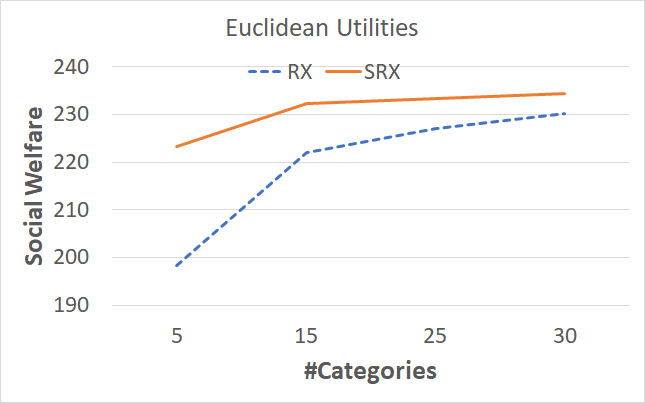
\includegraphics[width=6cm]{simulation/unit_cost_single_sw.png}
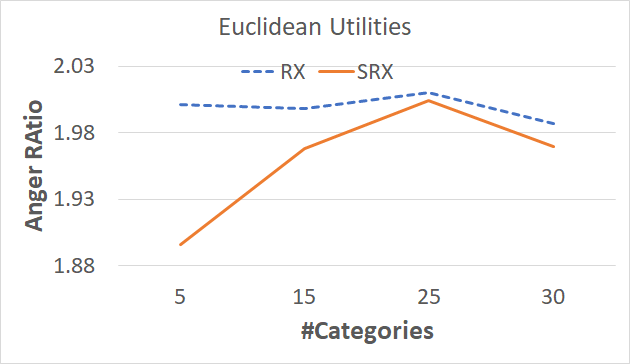
\includegraphics[width=6cm]{simulation/unit_cost_single_ar.png}
\caption{Left: Social welfare  of SRX and RX for different \#categories on euclidean utilities simulations~ (averaged over 1000 instances) with budget of 20. A higher value is better.\\
 Right: same comparison for the anger ratio. A lower value is better.
}\label{fig:type1}\vspace{-7.5mm}
\end{center}
\end{figure}

\begin{figure}[t]
\begin{center}
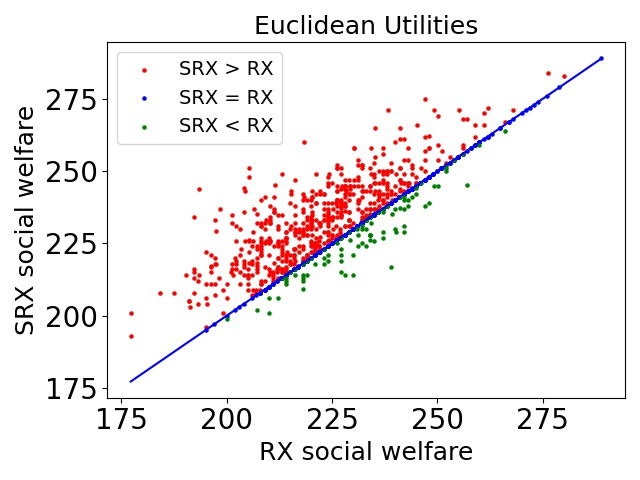
\includegraphics[width=6cm]{simulation/unit_cat(25)_bud(20).jpeg}
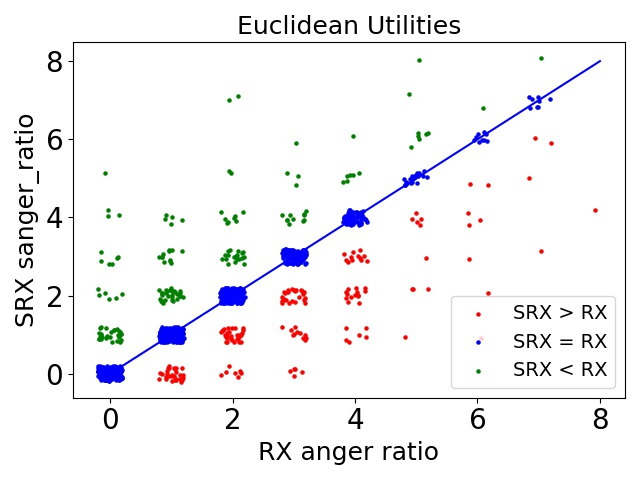
\includegraphics[width=6cm]{simulation/ar_unit_cat(25)_bud(20).jpeg}
\caption{Left: Achieved social welfare by SRX and RX for each of the 1000 instances.\\
Right: Achieved anger ratio by SRX and RX for each of the 1000 instances. Red instances when SRX performs better, green when RX performs better and blue for same value. \rmr{maybe flip so that green is better?}
 }\label{fig:scatter}\vspace{-7.5mm}
\end{center}
\end{figure}


% The  simulation results are  shown in Figures \ref{fig:type1} (for Type~1) and \ref{fig:type2} (for Type~2). 


Figure~\ref{fig:type1} shows how the SW and AR change as the number of categories is increasing (on average). As there are more categories, each voter will have less substitutes in their approved projects. This shows that on average SRX succeeds in achieving higher social welfare compared to RX in all of the scenarios. As the results trend was the same for all budget sizes, the figure shows the results only for budget of 20. Results for all budget sizes can be seen at Appendix~\ref{app:sim}.

As can be seen in the left graph of Figure~\ref{fig:type1}, SRX  achieves higher social welfare (on average) in more scenarios compared to RX. When looking at the anger ratio in the right graph of the figure, there are more "happy" voters (who get at least one project they wanted) compared to RX. In the global substitutes simulations the results were similar and can be seen in detail in Appendix~\ref{app:sim}.

% Figure~\ref{fig:type2} shows how the difference in SW and AR changes when letting the voters to approve different number of projects. As the results trend was the same for all cost distributions, the figure show the results only for cost distribution of N(300,20) (results for all budget sizes can be seen at Appendix~\ref{app:sim}).


% As can be seen in the top graphs of both figures, SRX succeeds to achieve higher social welfare (on average) in all scenarios compared to RX. When looking at the anger ratio in the bottom graphs of both figures, in the constant substitutes scenario there are more "happy" voters (who get at least one project they wanted) compared to RX. And in the unit cost scenario,  (bottom of Figure~\ref{fig:type1}) even though SRX satisfies the Strong-BPJR property, compared to RX which satisfies the stronger  EJR property, in most cases voters are more "happy" compared to RX, as determined by the anger ratio. 

One exception is when the budget is limited to 10 (Euclidean utilities), and RX succeeds in achieving  more happy voters (more details can be seen at Appendix~\ref{app:sim}).

When considering the   simulations in Figure~\ref{fig:type1}, we   see that as the number of categories of projects grow, the closer  the outcomes of RX and SRX become. This result makes sense as  more categories lead to  less  substitute projects and both mechanisms reach similar social welfare and anger ratio. 

Figure~\ref{fig:scatter} presents the results for the Euclidean utilities scenario with unit costs from a different perspective. This figure shows the achieved social welfare (left) and anger ratio (right) by SRX and RX for each of the 1000 instances, visualising how well each of them did compared to the other and in how many instances. As can be seen in the left plot, SRX succeed in achieving better social welfare in more cases compare to RX ($55\%$ vs $9\%$) Moreover, in the cases where SRX achieves better SW, the difference compared to RX is greater than the other way.

When looking at the right plot, there are about the same amount of cases for each rule which succeed in getting better anger ratio ($16\%$ SRX better and $15\%$ RX better). Actually, in the cases where the budget is 20, for all amount of categories the percentage of instances where each of the rules is better is very close to each other (where SRX have a bit more instances). This result is interesting, as anger ratio can also be thought of as a way to quantify how proportional an outcome is, and SRX succeed to compete with RX even through it holds weaker formal notion of proportionality in this scenario.

While Figure~\ref{fig:scatter} shows results only for 25 categories and budget of 20, other scenarios show the same trend. In addition, global substitutes simulations achieve even better results (having more instances where both the social welfare and anger ratio of SRX are better). More details about those cases can be seen in Appendix~\ref{app:sim}

% both plots, SRX succeed in achieving better social welfare in more cases compare to RX ($55\%$ vs $9\%$). Moreover, in the cases where SRX achieve better SW, the difference compare to RX is greater than the other way. The results were similar for different \#categories and budgets, as well for the Type~2 scenario. More details about those cases can be seen in Appendix~\ref{app:sim}

% Next, we  look at how the different scenarios affect the outcomes of the SRX mechanism.




% When considering the   simulations in  Figure~\ref{fig:type2}, we   see that as  voters are allowed to approve more projects, the difference in social welfare between SRX and RX increases. This also makes sense, since when voters approve more groups of substitute projects, SRX can achieve better social welfare by splitting the chosen projects between more groups. In contrast, the difference in anger ratio between SRX and RX decreases. In this case, only the voters that want completely different projects from the rest of the population will be hard to satisfy, therefore, there won't much difference between SRX and RX.

 
 One limitation of the simulations is that we chose very specific marginal utility function for substitute projects. If we would have used a different function for all partitions or different function for each partition, we might have gotten different results. %This leads to an interesting question, %\rmr{unclear: you want a more realistic description? I think this sentence can be removed}\rf{This sentence is about possible future study, what is the best marginal utility function to use in order to maximize proportionality \\ welfare} what is the best way to define the marginal utility functions for each of the partitions, which will give the best social welfare and proportionality guarantees.

%%%%%%%%%%%%%%%%%%%%%%%%%%%%%%%%%%%%%%%%%%%%%%%%%%%%%%%%%%%%%%%%%%%%%%%%

\section{Conclusion And Future Work}

\vspace{-7mm}
\begin{table}[ht!]
  \begin{center}
    \begin{tabular}{l|c|c|c|}
      & Global substitutes & Unit cost & General instances\\
      \hline
      SEJR & V & X & X\\
      SStrong-BPJR & V & V & X\\
    \end{tabular}
    \caption{\label{tab:prop}SRX proportionality summary (In which scenarios SRX holds proportionality)}
  \end{center}
\end{table}
\vspace{-7mm}

In this paper we proposed an input format that allows  voters to express substitute relationships over projects in PB.  
We extended the existing aggregation mechanism  Rule~X  to a new mechanism  SRX  that considers this input format. 
We showed that   SRX satisfies two notions of proportionality from the literature, summarised in Table~\ref{tab:prop}. First, it satisfies the Substitutes Extended Justified Representing (SEJR) notion of proportionality \cite{peters2020proportional} under global substitutes constraints in which all voters share the same partition over substitutes. Second,  it satisfies the SStrong-BPJR \cite{aziz2017proportionally} under conditions of    unit costs for projects but without requiring global substitutes. 

For both unit-cost and global substitutes scenarios  we created synthetic simulations that  satisfy   SEJR and SStrong-BPJR   proportionality. Our results show that the  SRX mechanism    achieves higher social welfare  than the RX mechanism in all scenarios while still maintaining  proportionality. In cases where SRX holds a weaker notion of proportionality than rule RX, SRX  still succeeds in lowering voters' ``anger ratio" i.e.,   more voters receive at least one project they want.

There are several directions we plan for future research:
First, we wish to define new notions of  proportionality for the case of substitute projects that will guarantee the voters some utility, rather than the  number of projects (using the marginal utilities).
Second, while this paper focused on proportionality guarantees for SRX, we will study what guarantees it possible to get for the social welfare.
This will be followed with far extensive simulations which will include further analysis of SRX using different marginal utility functions and comparing to more mechanisms from the literature, even when proportionality doesn't hold.
Lastly, we will study different family of marginal utility functions that can give better guarantees for both proportionality and social welfare.

\rf{Added the paragraph about the EJR extension}
Finally, one might argue how natural is the extension that was chosen for SEJR in the substitutes case. Using the current definition, proportionality gives a guarantees on number of funded projects, however, it doesn't guarantee anything about the utility a voter might get. Therefore, it will be interesting to find a more natural extension to SEJR, which might require to find new mechanism that will hold it.

%%%%%%%%%%%%%%%%%%%%%%%%%%%%%%%%%%%%%%%%%%%%%%%%%%%%%%%%%%%%%%%%%%%%%%%%
%
% ---- Bibliography ----
%
% BibTeX users should specify bibliography style 'splncs04'.
% References will then be sorted and formatted in the correct style.
%
\begin{small}
\bibliographystyle{splncs04nat}
%\bibliographystyle{plain}

\bibliography{ref.bib}
%
\end{small}
%%%%%%%%%%%%%%%%%%%%%%%%%%%%%%%%%%%%%%%%%%%%%%%%%%%%%%%%%%%%%%%%%%%%%

\clearpage
\begin{subappendices}

\section{Q Value Full Algorithm}\label{app:qval}

\begin{algorithm}[h]
\SetAlgoLined
\textbf{Input:} 
\begin{enumerate}
    \item project $p\in A$ \\ 
    \item $\forall i\in V,  U_i(p)$ \\
    \item $\forall i\in V,  b_i(t)$ \\
    
\end{enumerate}
\KwResult{The qValue of project $p$}
\If {$\sum_{i\in v, U_i(p)>0}b_i(t)< cost(p)$}
 {$return \  \infty$}
 
 $current\_utility \leftarrow \sum_{i\in V}U_i(p)$
 
 $cost\_leftover \leftarrow cost(p)$
 
 $removed\_voters \leftarrow \varnothing$
 
 \While{True}{
    $current\_q \leftarrow cost\_leftover /    current\_utility$
    
    $voter\_removed \leftarrow False$
    
    \For{$i\in V\setminus removed\_voters$}{
      \If{$current\_q \cdot U_i(p) > b_i(t)$}{
            $current\_utility \leftarrow current\_utility - U_i(p)$
            
            $cost\_leftover \leftarrow cost\_leftover - b_i(t)$
            
            $removed\_voters \leftarrow removed\_voters \cup \{i\}$
            
            $voter\_removed \leftarrow True$
       }
       
     }
     
     \If{$voter\_removed == False$}{
            $return \  (cost\_leftover / current\_utility)$
       }
 }

 \caption{qValue}
\end{algorithm}


\section{Additional Proofs and notes}\label{app:proofs}

% Proof for Theorem~\ref{theorem:spr}:
% \begin{proof}
% Given PB scenario E, some $\ell\in \{1,\ldots,L\}$ and $S\subseteq V$  we  assume towards a contradiction that there is some $T\subseteq A$ which all voters in $S$ approve all projects in $T$ and no other project and it holds that $|T\cap R(E)|<|T|$ and $\exists p\in T\setminus R(E), cost(p) +cost(T\cap R(E))\leq \ell$.


% We can look at two cases:
% \begin{enumerate}
%     \item $cost(T)\leq\ell$ - in this case voters $S$ can fund all projects in $T$. Its given that SRX stops with $|T\cap R(E)|<|T|$, but since we know from SRX definition they can't fund projects not from $T$ (as they didn't approved them), it holds that $T\cap R(E)\subset T$. This in that project $p$ still can be funded, in contradiction that SRX stopped.
    
%     \item $cost(T)>\ell$ - This mean that group $S$ can't fund all projects in $T$, so it holds that $|T\cap R(E)|<|T|$. From assumption there is some project $p\in T$ such that $cost(p) +cost(T\cap R(E))\leq \ell$ when SRX stops, however, since group $S$ doesn't fund any project outside of $T$, it means that project $p$ can be funded by voters in $S$, in contradiction that SRX stopped
% \end{enumerate}
% \end{proof}

% The requirement that  marginal utilities are non zero is necessary: if in the set of projects $T$ we have substitute projects, funding one of them will make some of the voters not wanting the other items anymore, resulting with only part of $T$ being funded.

% However this requirement can sometimes be relaxed. In fact we only require that for any group of voters $S$ such as defined for SPR, their marginal utilities will be defined such they will want (having non zero utility) all projects in $T$. Formally, in addition to requesting that all voter in $S$ approve all projects in $T$ and no other project, we request that $\forall i\in S, \forall g\in v_i, u_{i,g}(k)>0 $ for all $k\leq |g\cap T|$.

% In addition, in many cases it actually desirable for the marginal utility to be non zero. This is because it can cause cases where there is some project that several voters want it to be funded (some with utility 0 as it is substitute to some funded project), there is enough budget for it, but it won't be funded. While one might claim that it's not funded because the voters don't want a substitute project, it raise the question whether a PB mechanism should exhausts its entire budget or leave some of the budget unused.


Proof for Theorem~\ref{theorem:unit}:

\begin{proof}
First, lets notice that at each step SRX have two options to choose a project $p\in A\setminus B_t$, either $p$ not approved by any voter in $S$ or approved by at least one voter $i\in S$.

If $p$ is  not approved by any voter in $S$, it mean that the funds group $S$ have, hasn't changed, so we can ignore this step and look at the next one. If $p$ was approved by some voter $i\in S$, then happen two important things. First, the group $S$ of voter used at most 1 from their total funds in order to fund $p$, this is because all projects are unit cost. Secondly, Since $i\in S$ approved $p$, it means that $|\cup_{i\in S}A_i\cap B_t|$ increased by one.

This mean that in each step, either group $S$ didn't used their funds or they used at most 1 and they got one more approved project. But since group $S$ is T-cohesive, it means that their initial funds are at least $|T|$, this mean that in order to finish their funds they must have funded at least $|T|$ projects, which mean that $|\cup_{i\in S}A_i\cap B_t|\geq |T|$.\qed
\end{proof}

\section{Simulation}\label{app:sim}



\begin{figure}[t]
\begin{center}
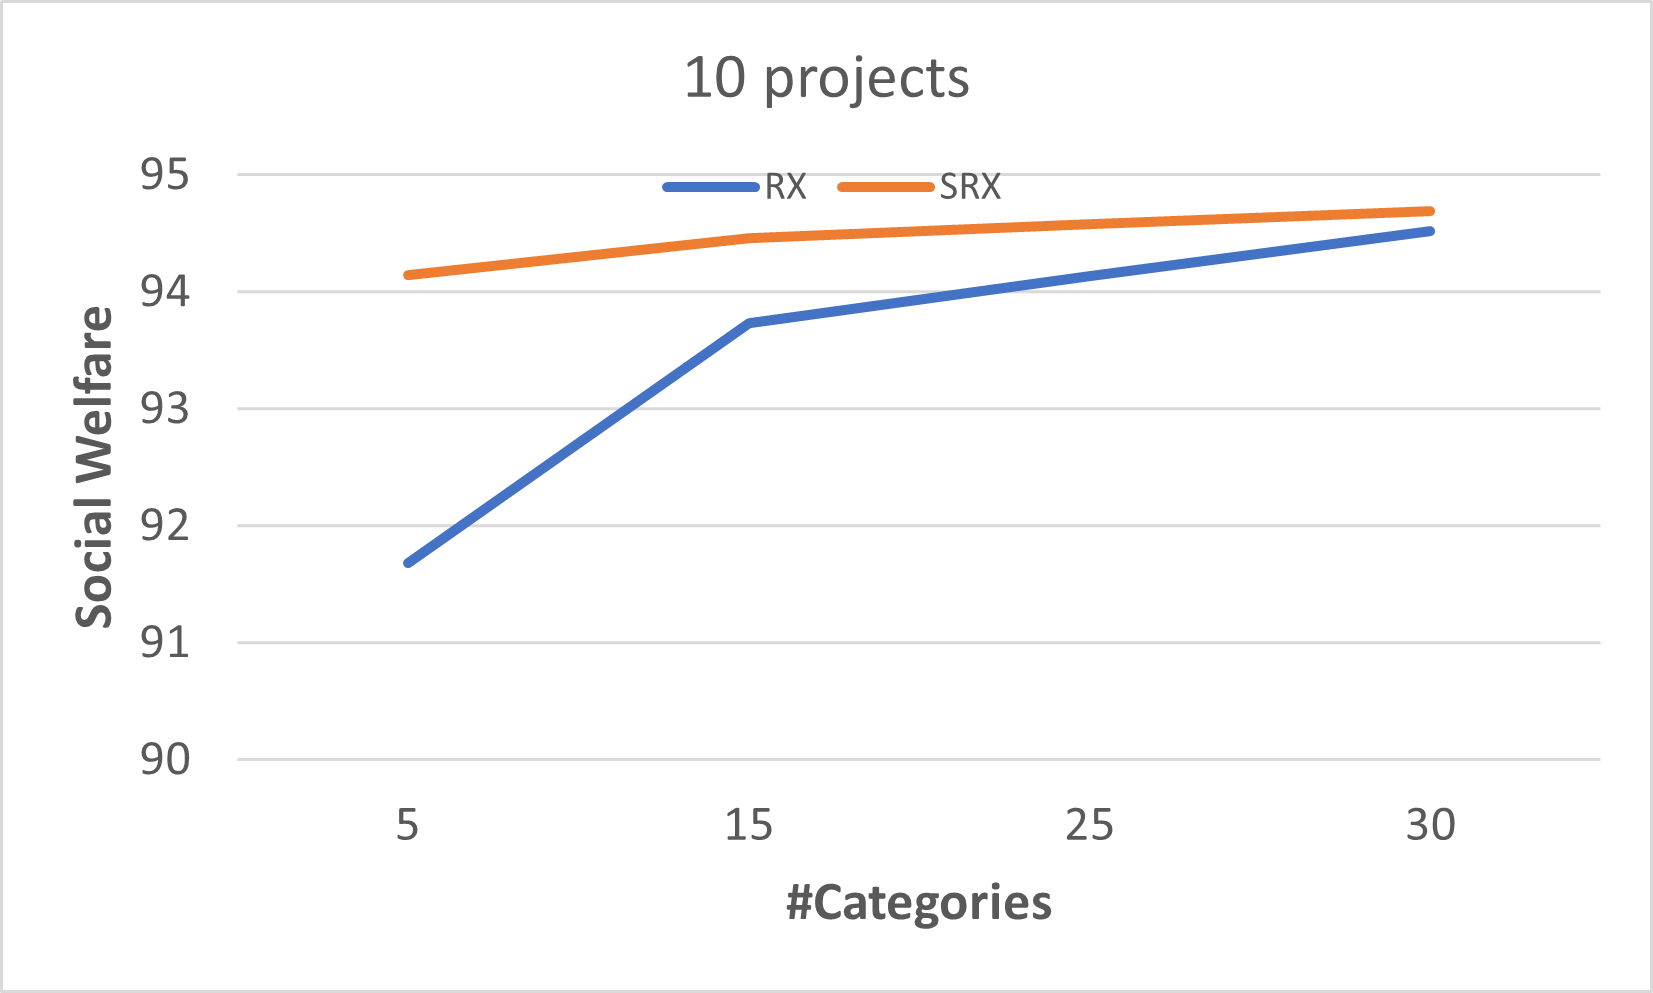
\includegraphics[width=6cm]{simulation/unit_cost_sw_10.png}
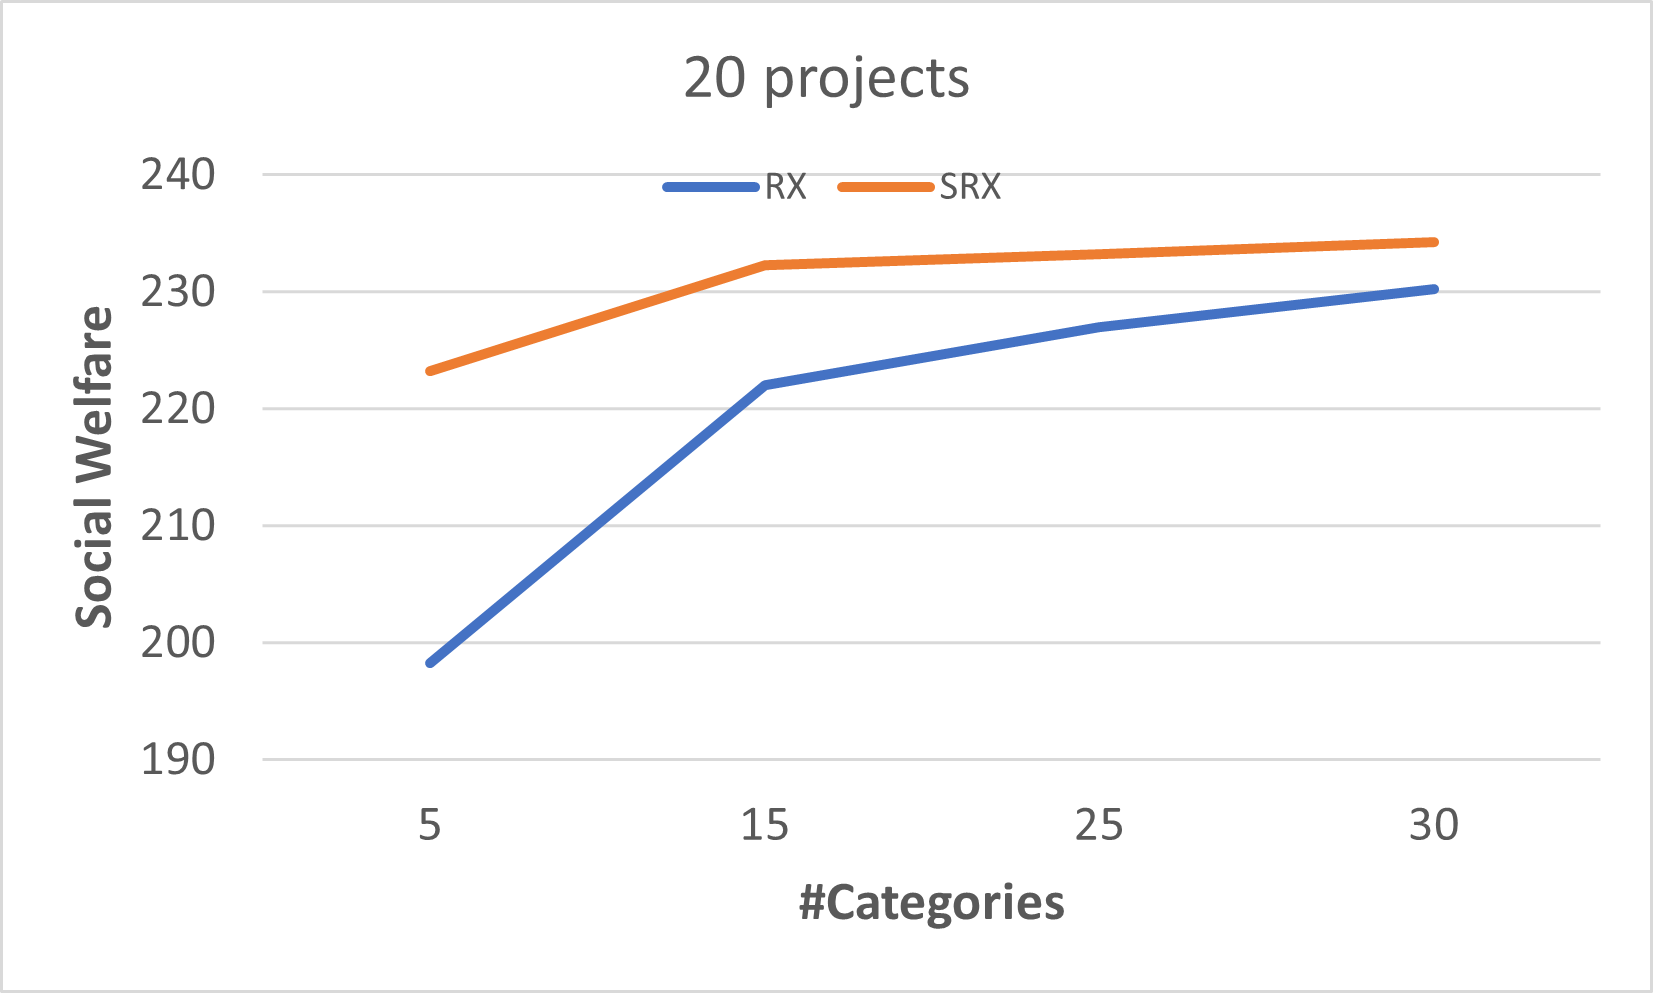
\includegraphics[width=6cm]{simulation/unit_cost_sw_20.png}
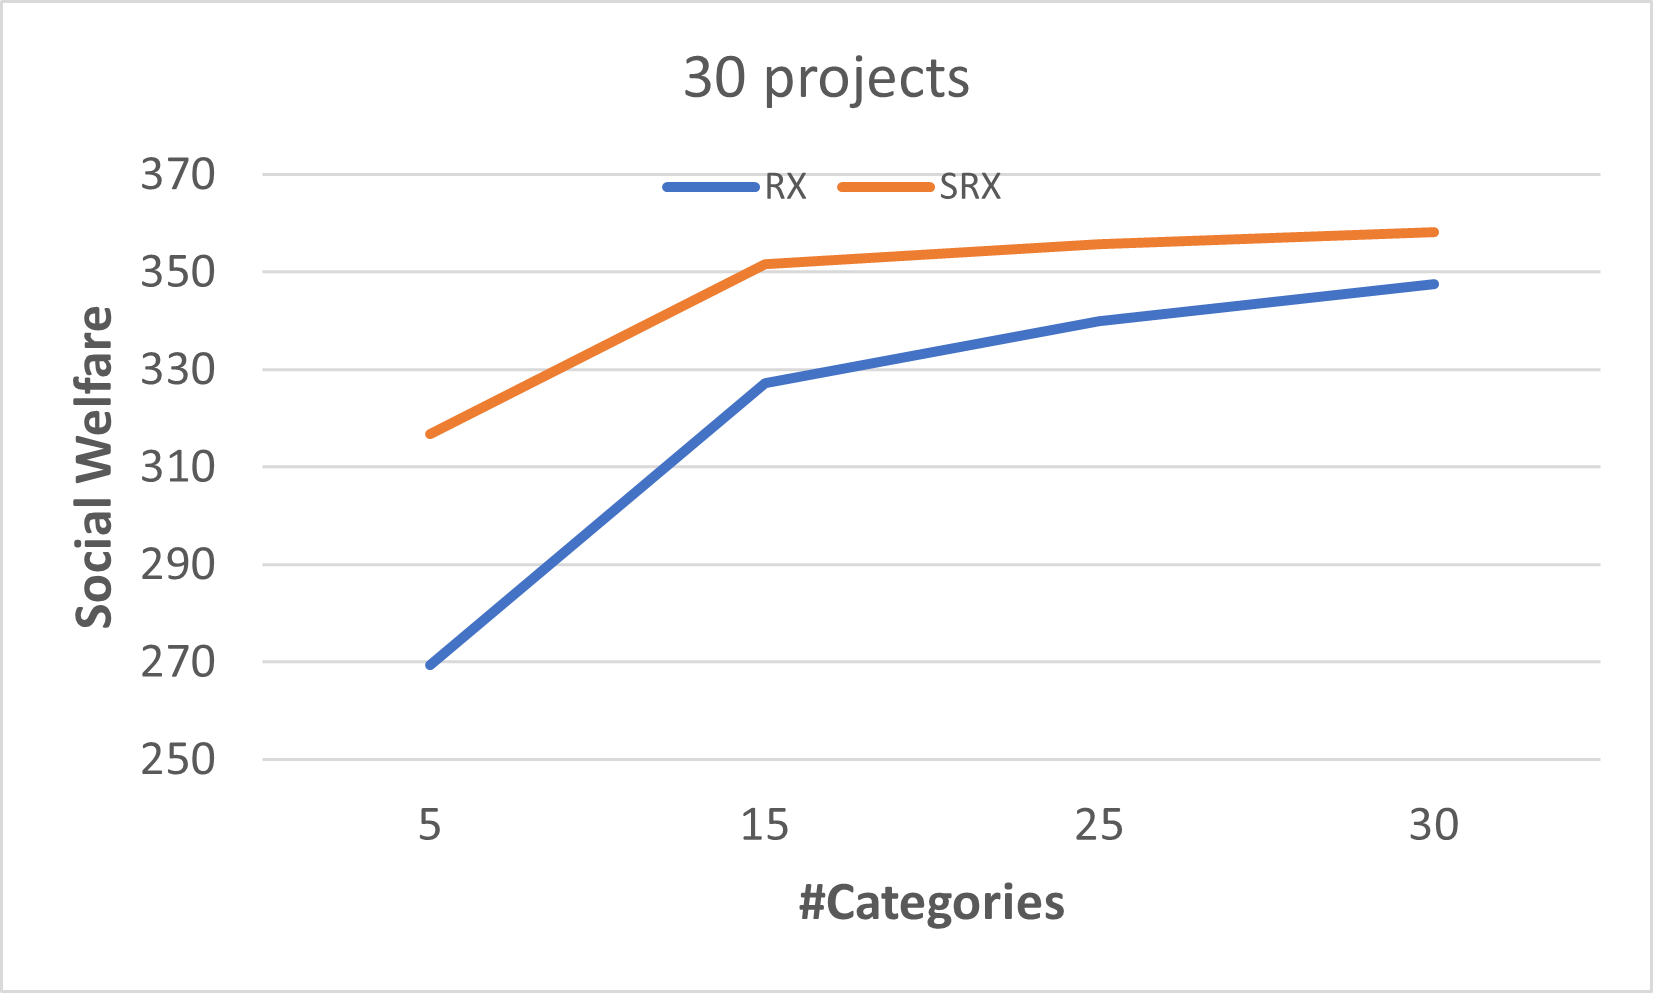
\includegraphics[width=6cm]{simulation/unit_cost_sw_30.png}
\caption{Average social welfare achieved by RX and SRX for different size of budget in Euclidean utilities simulations.
}\label{fig:sw_all1}
\end{center}
\end{figure}

\begin{figure}[t]
\begin{center}
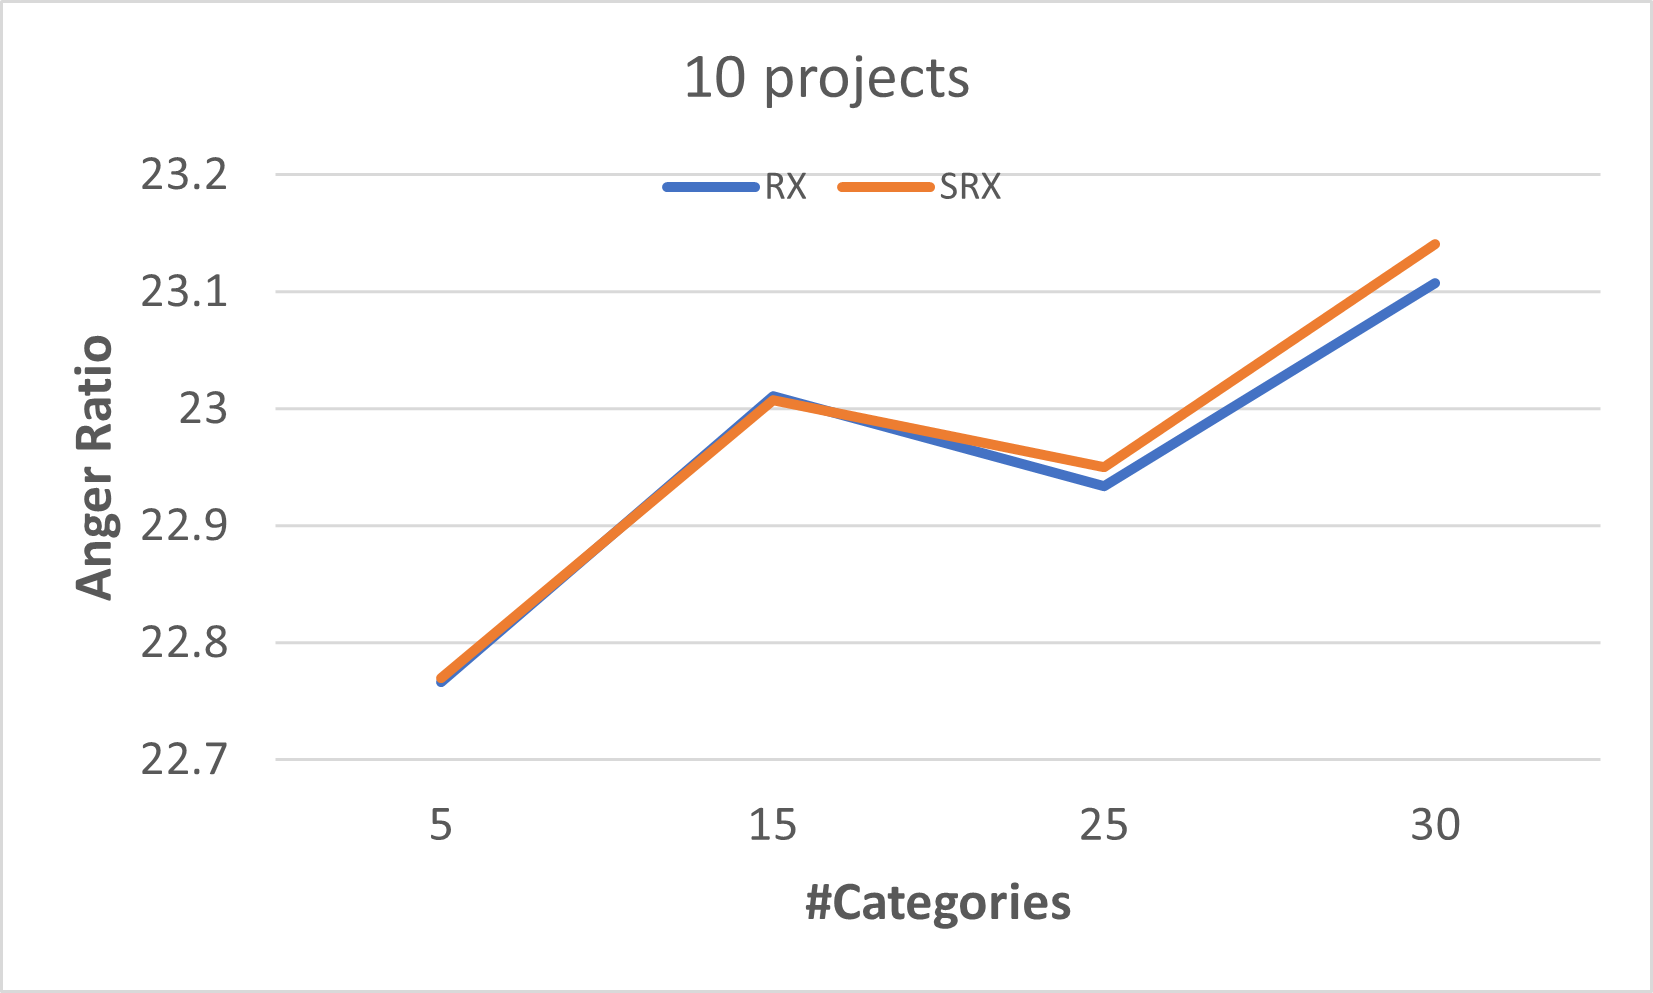
\includegraphics[width=6cm]{simulation/unit_cost_ar_10.png}
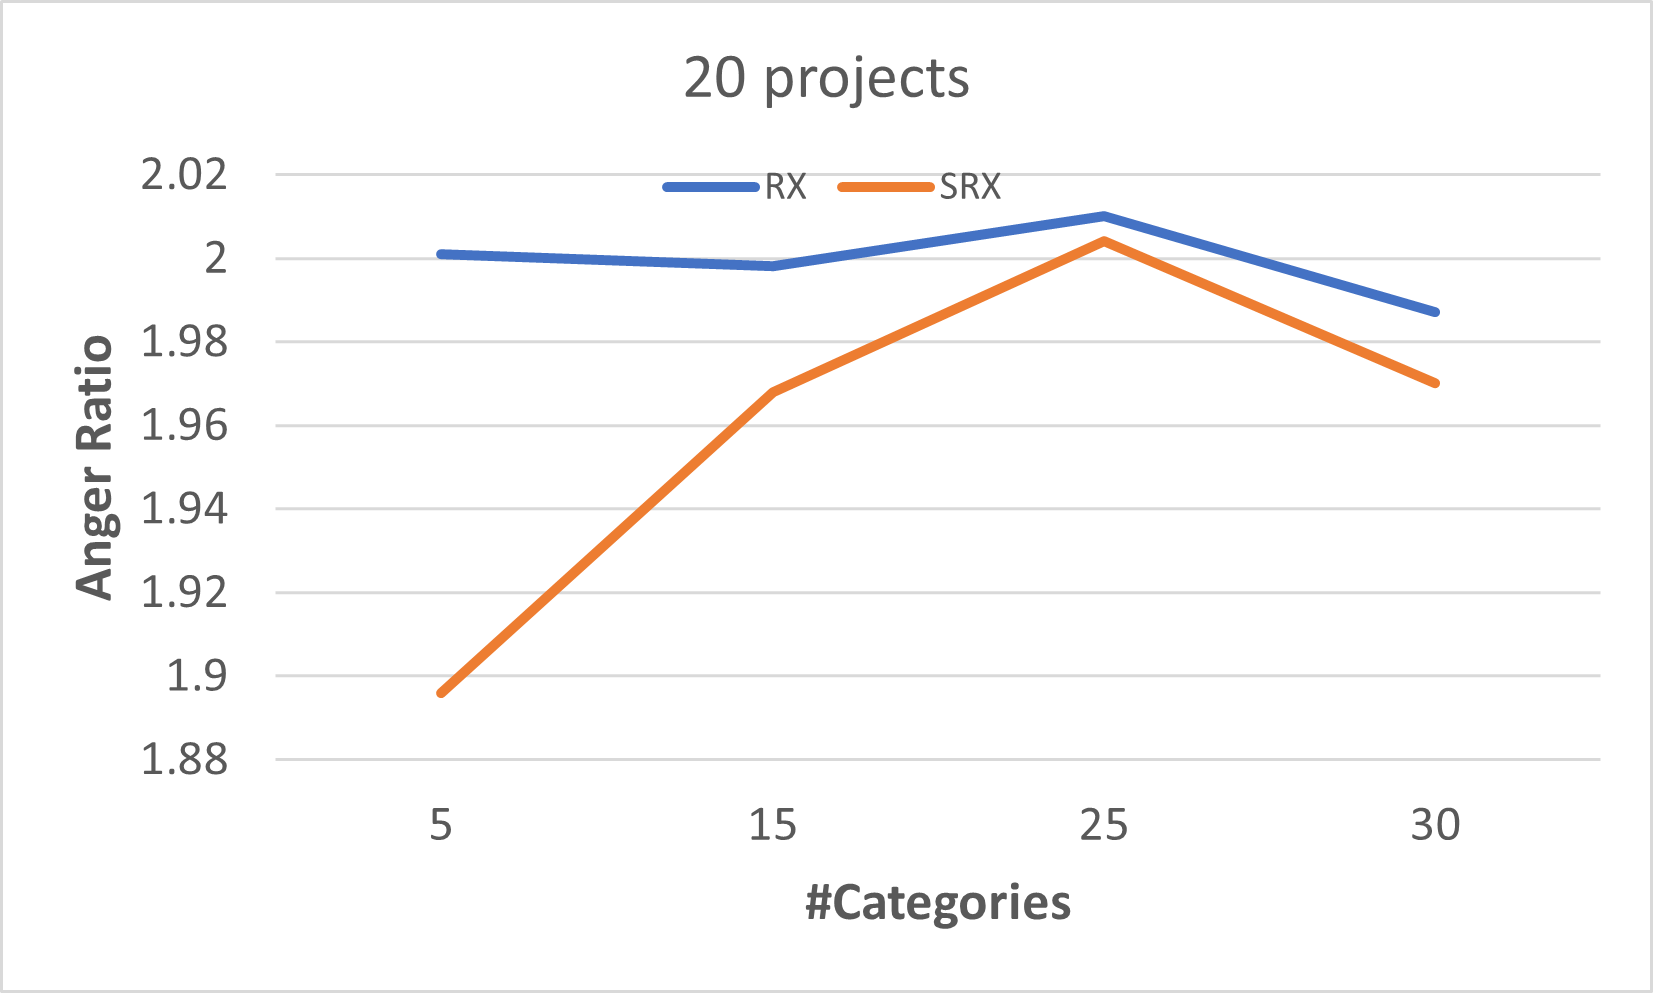
\includegraphics[width=6cm]{simulation/unit_cost_ar_20.png}
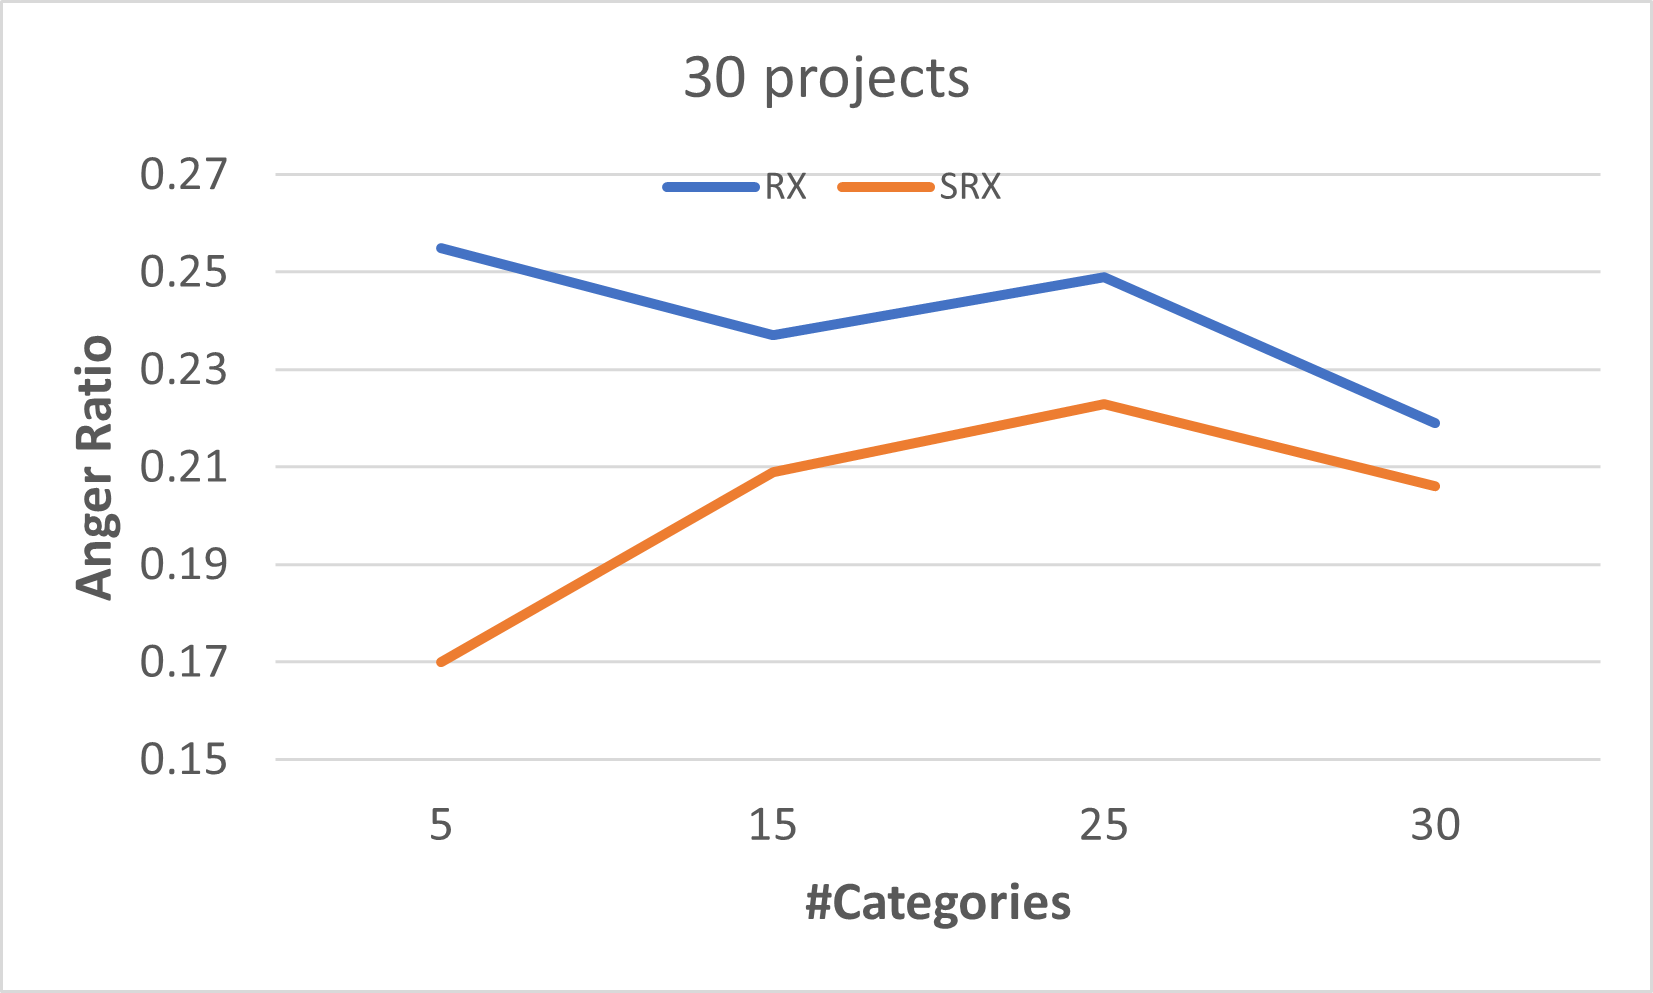
\includegraphics[width=6cm]{simulation/unit_cost_ar_30.png}
\caption{Average anger ratio achieved by RX and SRX for different size of budget in Euclidean utilities simulations.
}\label{fig:ar_all1}
\end{center}
\end{figure}

% Figure~\ref{fig:type2} shows how the difference in SW and AR changes when letting the voters to approve different number of projects. As the results trend was the same for all cost distributions, the figure show the results only for cost distribution of N(300,20) (results for all budget sizes can be seen at Appendix~\ref{app:sim}).

% When considering the   simulations in  Figure~\ref{fig:type2}, we   see that as  voters are allowed to approve more projects, the difference in social welfare between SRX and RX increases. This also makes sense, since when voters approve more groups of substitute projects, SRX can achieve better social welfare by splitting the chosen projects between more groups. In contrast, the difference in anger ratio between SRX and RX decreases. In this case, only the voters that want completely different projects from the rest of the population will be hard to satisfy, therefore, there won't much difference between SRX and RX.

Figure~\ref{fig:sw_all1} and Figure~\ref{fig:ar_all1} Shows how the size of the project in Euclidean utilities simulations affect the social welfare and anger ratio achieved by RX and SRX. As expected the gap between SRX and RX is getting larger as there is a bigger budget, this is because when there is a small budget there isn't a chance to decide between two projects where one of them is substitute to another funded project. Need to say, that in the case where the budget is too small for utilize the advantage of substitutes, RX succeed in achieving better anger ratio (not with big margin).

Figure~\ref{fig:sw_all2} and Figure~\ref{fig:ar_all2} shows how the difference in SW and AR changes when letting the voters to approve different number of projects and using different cost distribution for the projects in global substitutes simulations.

When considering those   simulations , we   see that as  voters are allowed to approve more projects, the difference in social welfare between SRX and RX increases. This also makes sense, since when voters approve more project partitions, SRX can achieve better social welfare by splitting the chosen projects between more partitions. In contrast, the difference in anger ratio between SRX and RX decreases. In this case, only the voters that want completely different projects from the rest of the population will be hard to satisfy, therefore, there won't much difference between SRX and RX.


In addition when looking at the effect of different cost distribution, the lower the $\sigma$ chosen for the cost, the higher the difference in voter satisfaction and the lower the difference in anger ratio. This happens because the bigger the $\sigma$ is, there are more cheaper projects, this way it is easier to ignore the the expensive ones and look only the cheap, helping avoid the need to choose between cheap substitute project compared to expensive not substitute project. Lastly, we didn't saw any significant change when using different mean for the cost, therefore, the figure shows only for mean=300.

\begin{figure}[t]
\begin{center}
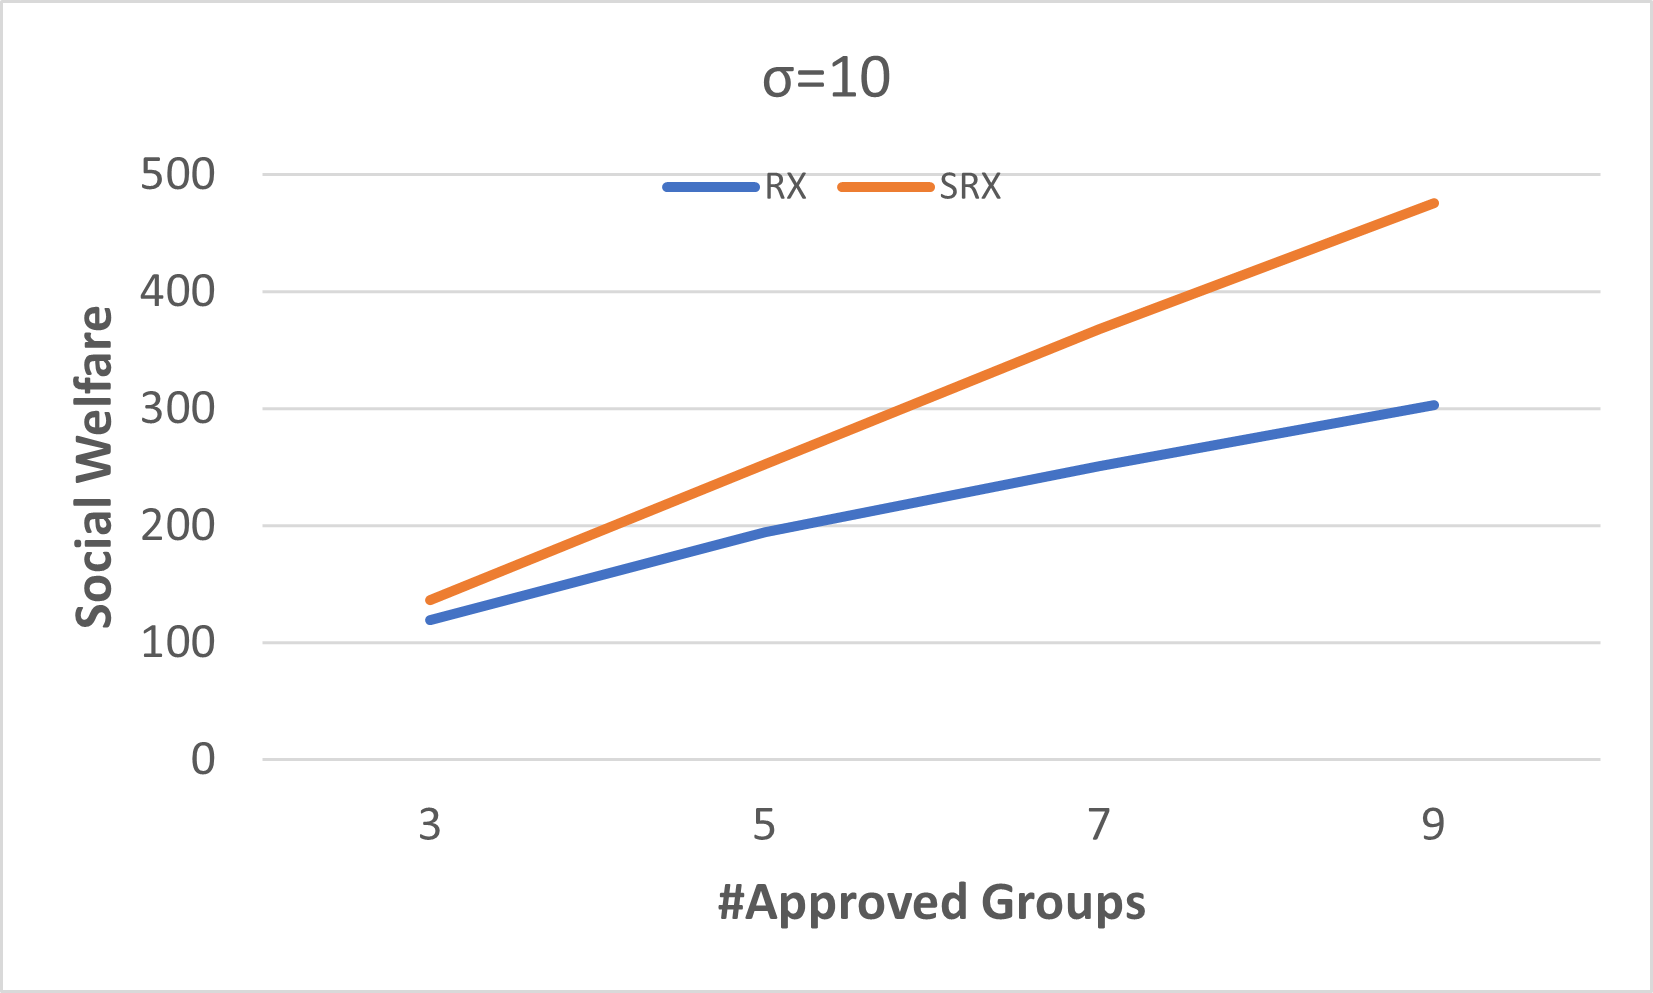
\includegraphics[width=6cm]{simulation/constant_substitutes_sw_10.png}
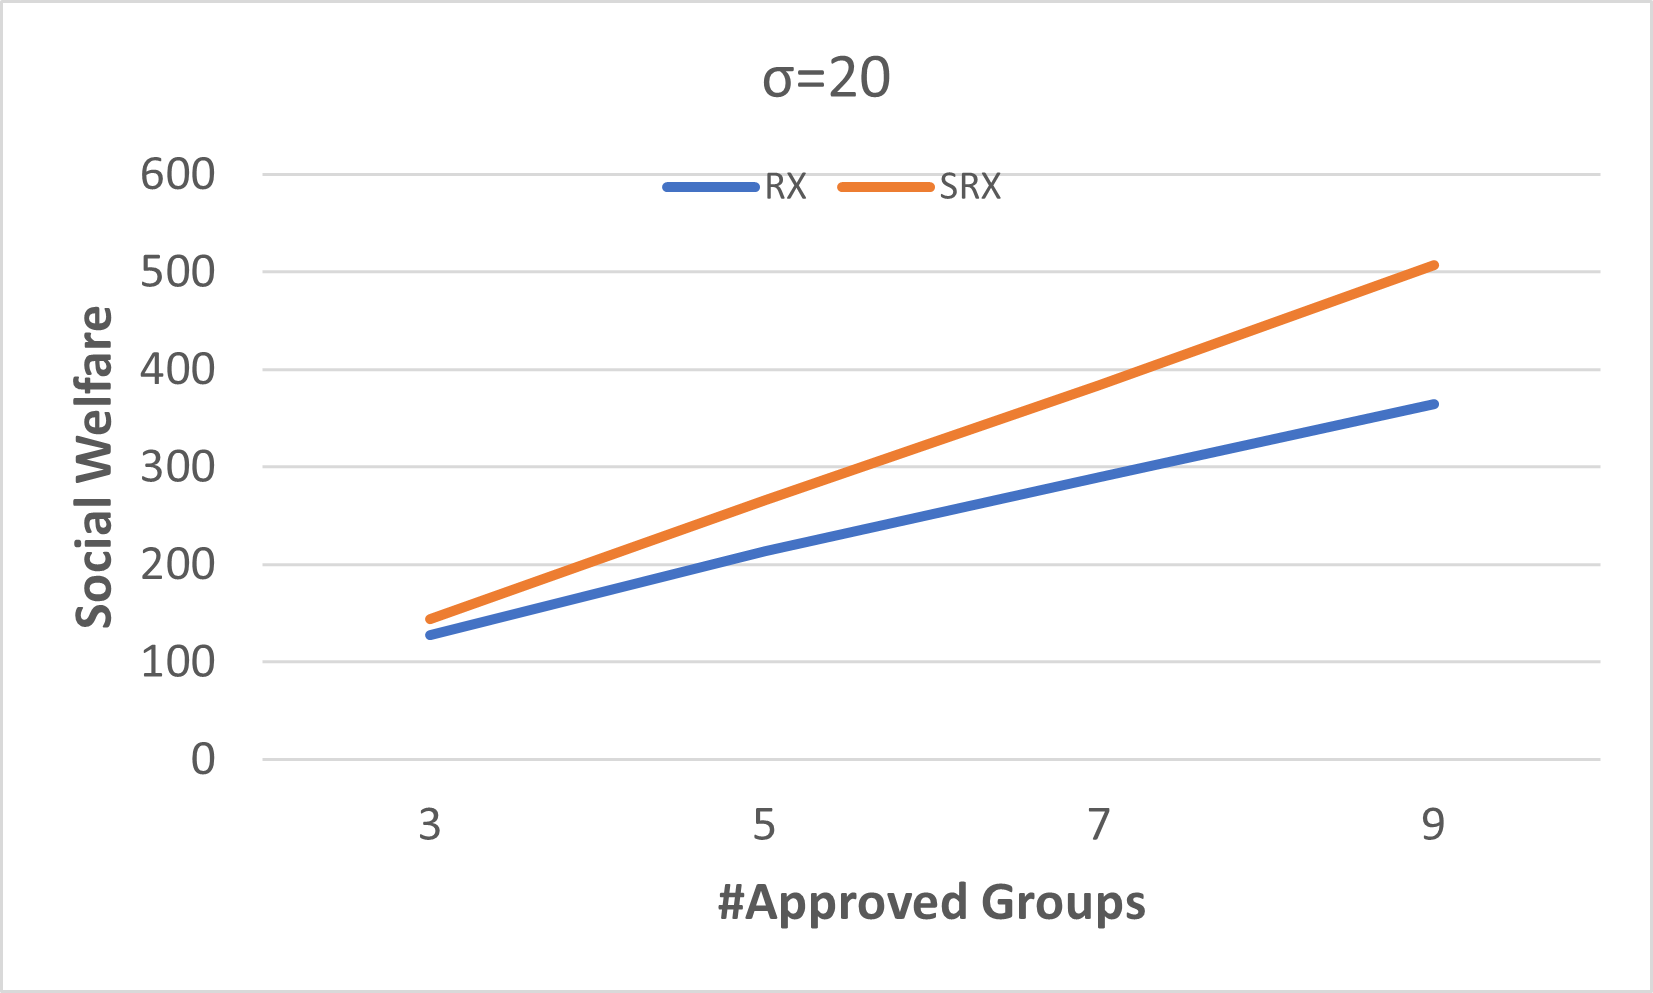
\includegraphics[width=6cm]{simulation/constant_substitutes_sw_20.png}
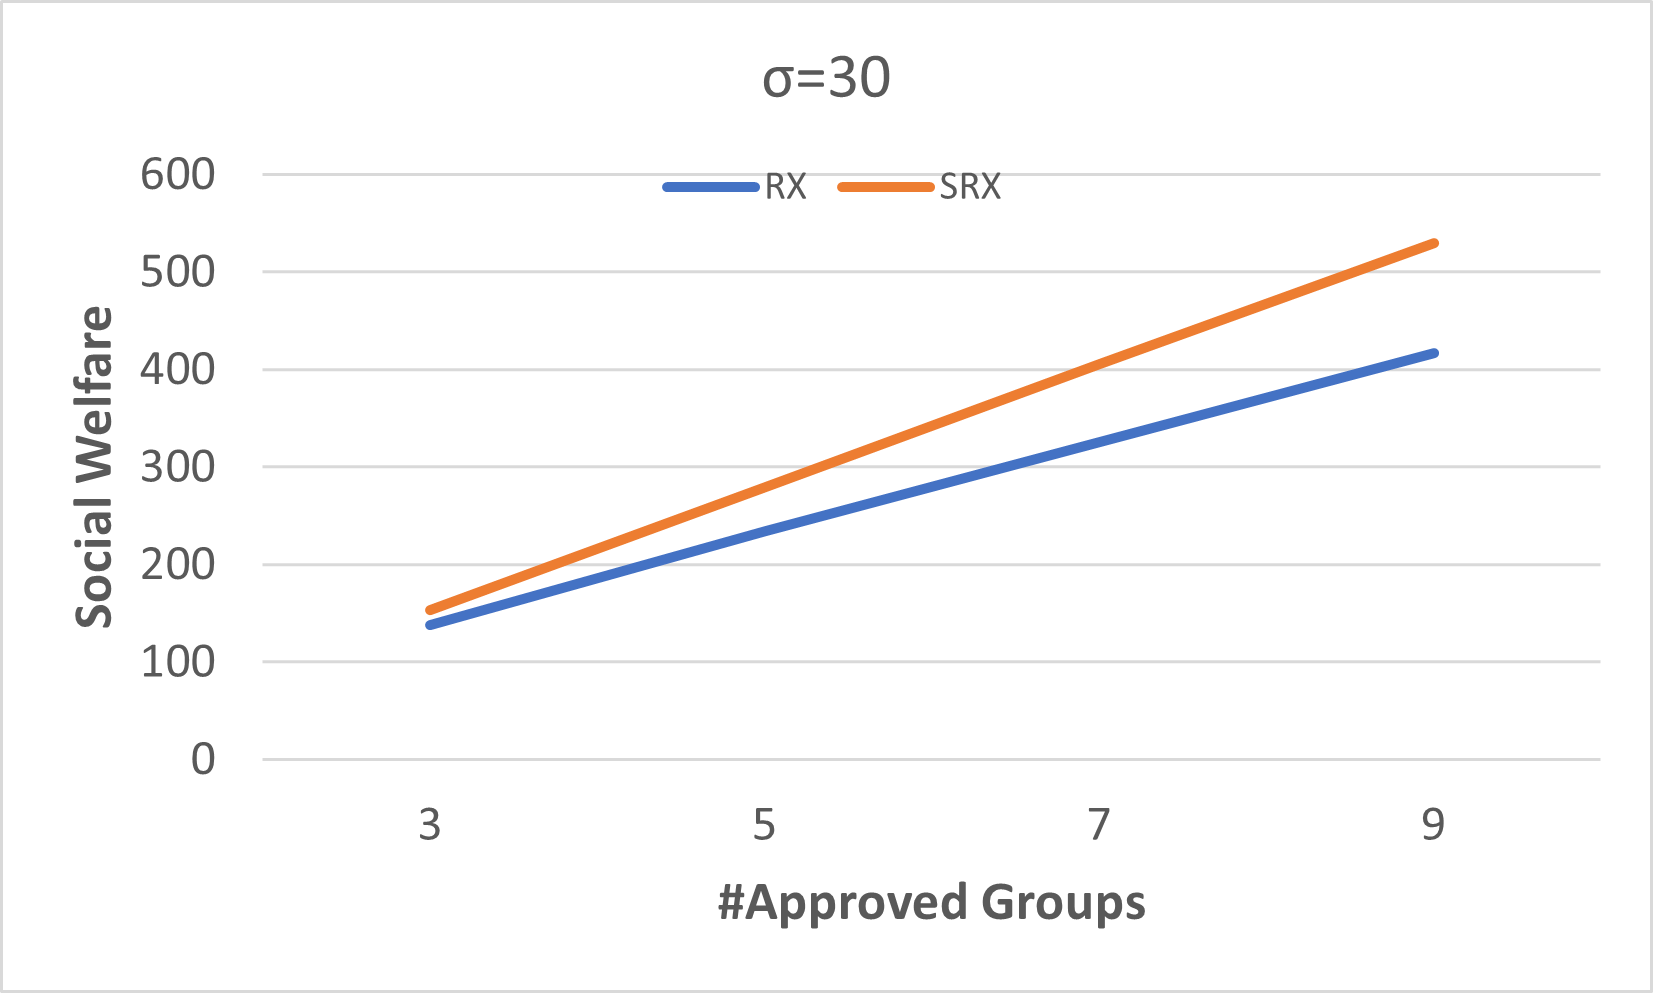
\includegraphics[width=6cm]{simulation/constant_substitutes_sw_30.png}
\caption{Average social welfare achieved by RX and SRX for different cost distribution in global substitutes simulations.
}\label{fig:sw_all2}
\end{center}
\end{figure}


\begin{figure}[t]
\begin{center}
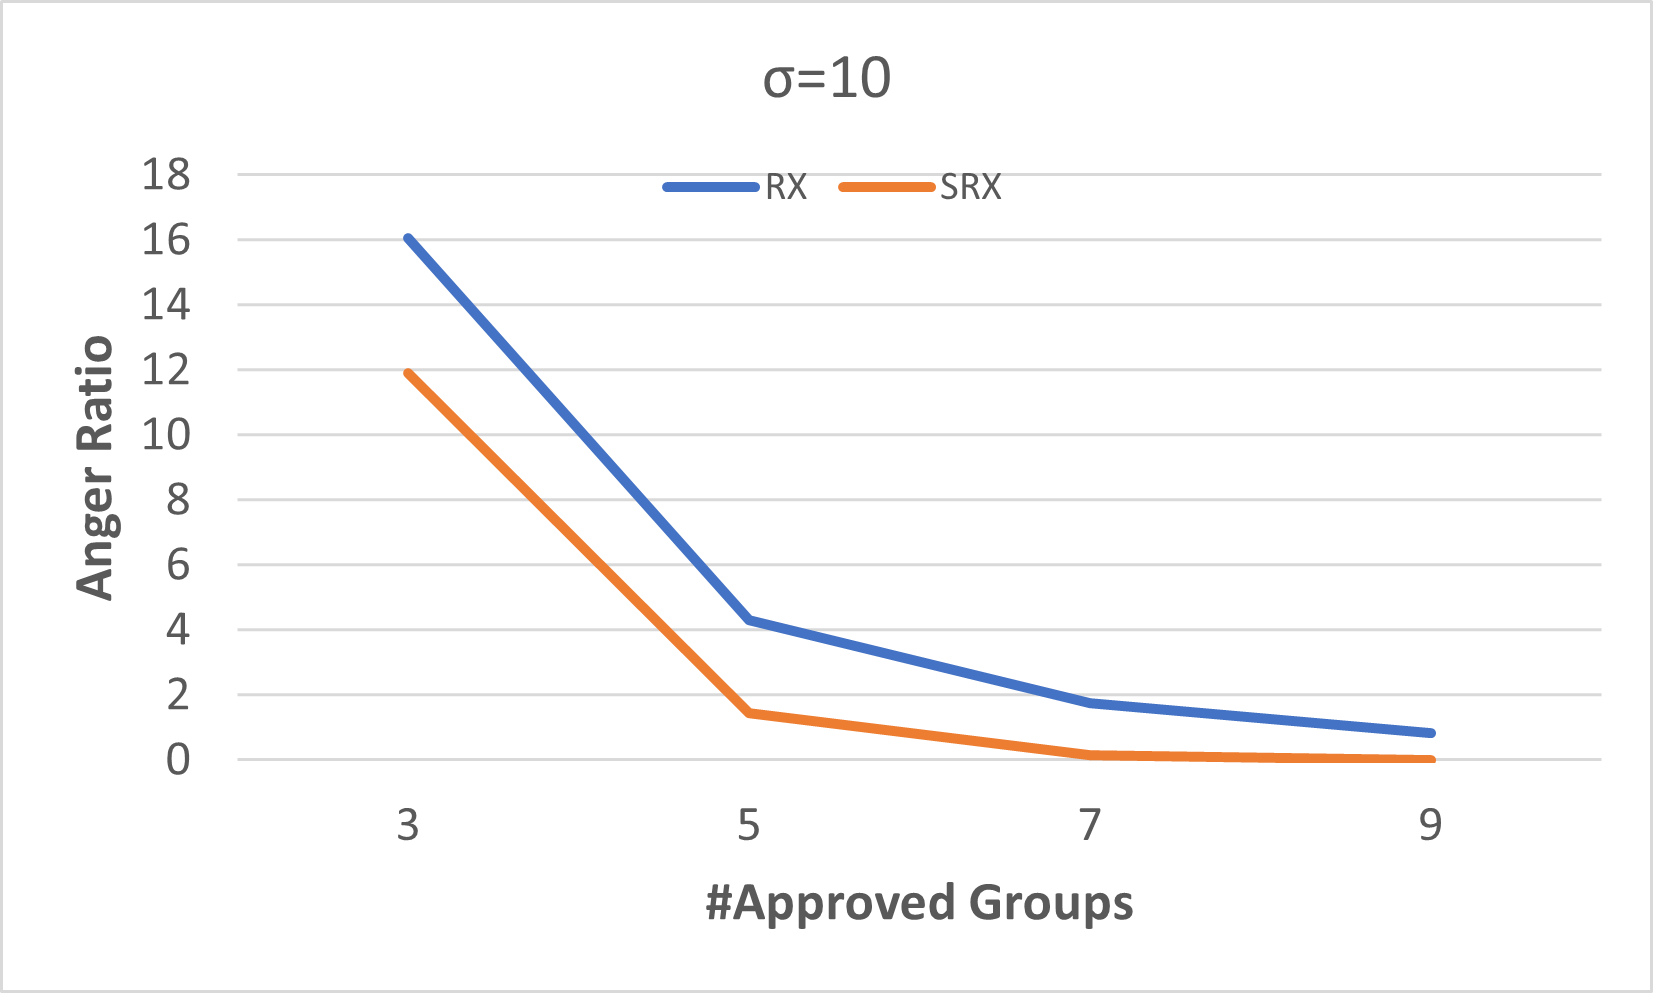
\includegraphics[width=6cm]{simulation/constant_substitutes_ar_10.png}
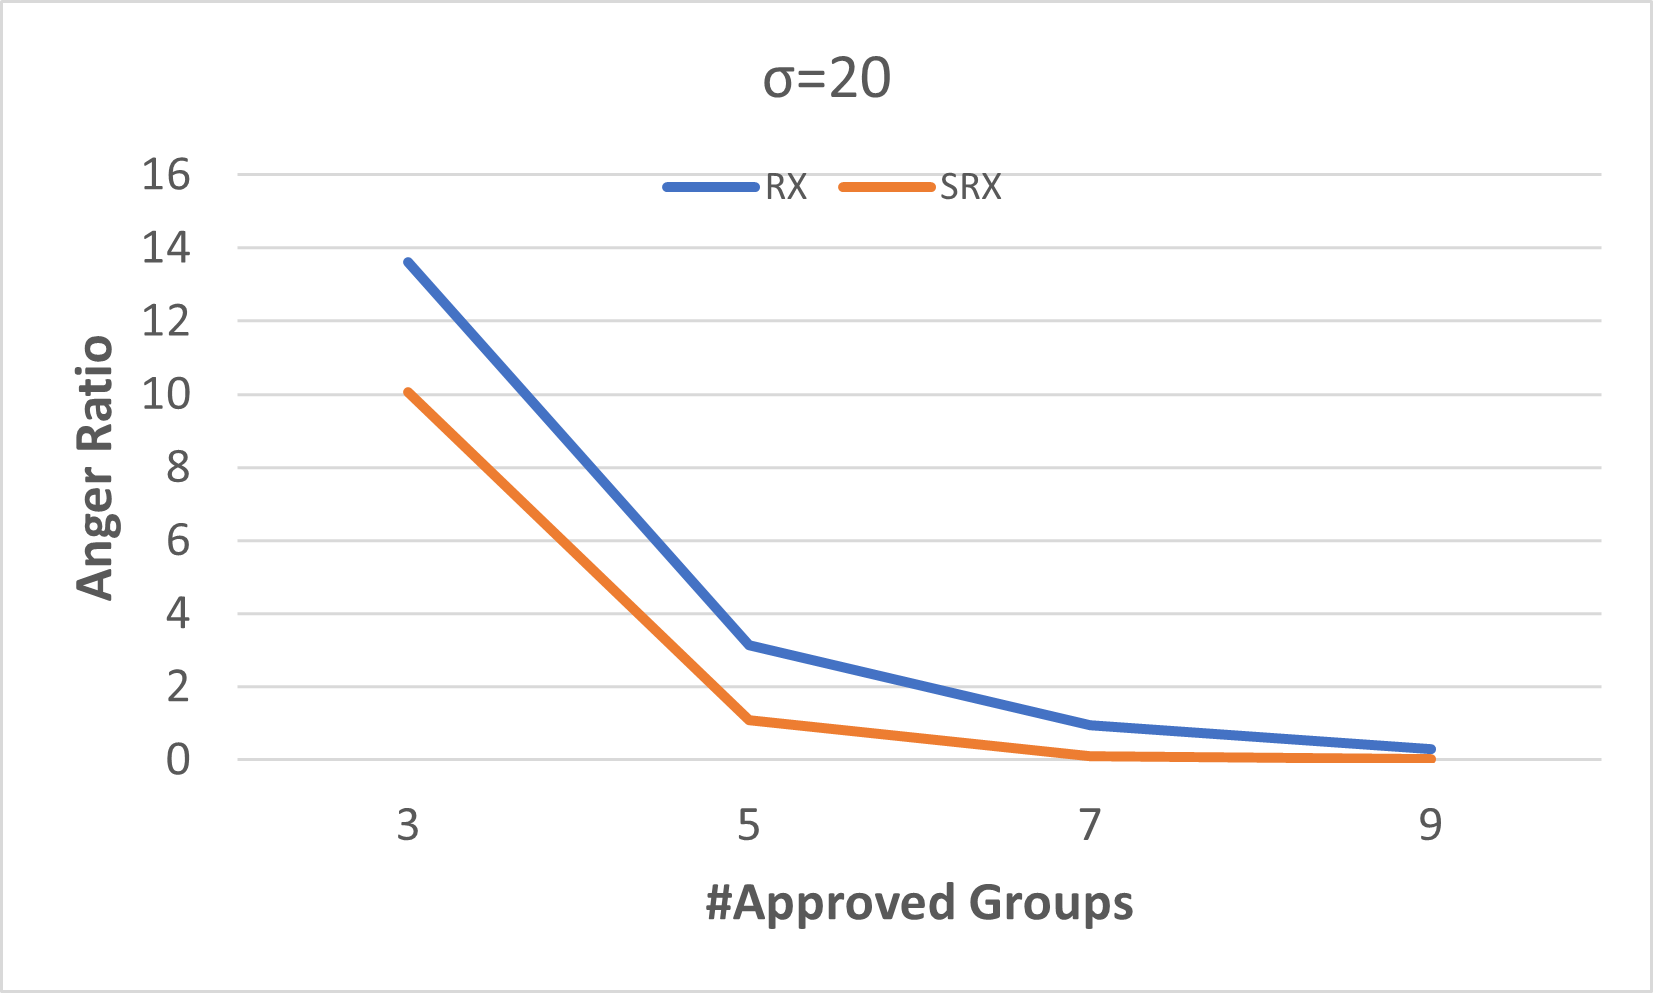
\includegraphics[width=6cm]{simulation/constant_substitutes_ar_20.png}
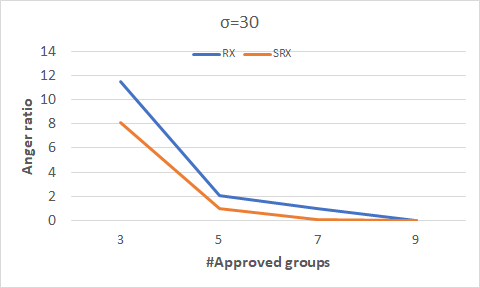
\includegraphics[width=6cm]{simulation/constant_substitutes_ar_30.png}
\caption{Average anger ratio achieved by RX and SRX for different cost distribution in global substitutes simulations.
}\label{fig:ar_all2}
\end{center}
\end{figure}

Figure~\ref{fig:scatter_all1} and Figure~\ref{fig:scatter_all2} better demonstrates the social welfare SRX and RX succeed achieving in both types of simulations. As mentioned in Section~\ref{sec:exp}, SRX succeed in achieving better social welfare in most instances. In addition the difference in social welfare when SRX is better is bigger than the other way. This is especially notable in Figure~\ref{fig:scatter_all2} where the few instances where RX is better, the difference in SW is pretty much negligible.

When look at the results from the unit cost scenario, it possible to better notice the effect of \#categories and the budget. First, when the budget is small, there isn't a lot of place to "manipulate" the outcome, and in most cases both mechanism result with the same SW. When the budget increase the more power SRX has when considering substitute projects, this is why there are more instances where SRX get better SW than RX when the budget 30 compared to 20.

When looking how the number of categories affect the social welfare, as said in Section~\ref{sec:exp}, SRX are RX are getting closer results as the effect of substitute projects become less meaningful.

Lastly, in Figure~\ref{fig:scatter_all2}, it is possible to see that SRX is better in almost all instances, and even when RX is better, it is by a small difference. This results is especially interesting due the fact that in global substitutes simulations, SRX holds SEJR in all instances, same as RX. This show that SRX can achieve better outcomes compared to RX without losing level of proportionality in the process.

Figure~\ref{fig:scatter_all_ar1} and Figure~\ref{fig:scatter_all_ar2} better demonstrates the anger ratio SRX and RX succeed achieving in both types of simulations. As mentioned in Section~\ref{sec:exp}, SRX have very close percentage of instances where it achieve better anger ratio to percentage RX achieve.

Looking more closely at Figure~\ref{fig:scatter_all_ar1}, it possible to better notice the effect of \#categories and the budget. Both when the number of categories increase and the budget decrease, SRX and RX are getting more similar anger ratios. This happen because when the number of categories increase, each voter will have less substitutes and the effect of SRX will be more negligible. In addition when having smaller budget, SRX can have less option to "manipulate" the outcome, as it is not enough to fund many substitutes.

Figure~\ref{fig:scatter_all_ar2} demonstrate the disadvantage of relying on SEJR, since there are cases where this definition is problematic. This is because it is possible to hold SEJR when a very small amount of voters get several projects they want, while the rest of population doesn't receive any project at all. The measurement of anger ratio present this well as can be seen in the Figure~\ref{fig:scatter_all_ar2}. In this scenario, both SRX and RX hold SEJR, meaning they both are proportional, however, SRX have much more instances where every (or less voters compared to RX) voter get at least one project he wanted.

The results from the simulations help to show that SRX compete well against RX. It succeeds in achieving better social welfare, while still satisfying big part of the voters, even in cases where it doesn't hold SEJR.


\begin{figure}[t]
\begin{center}
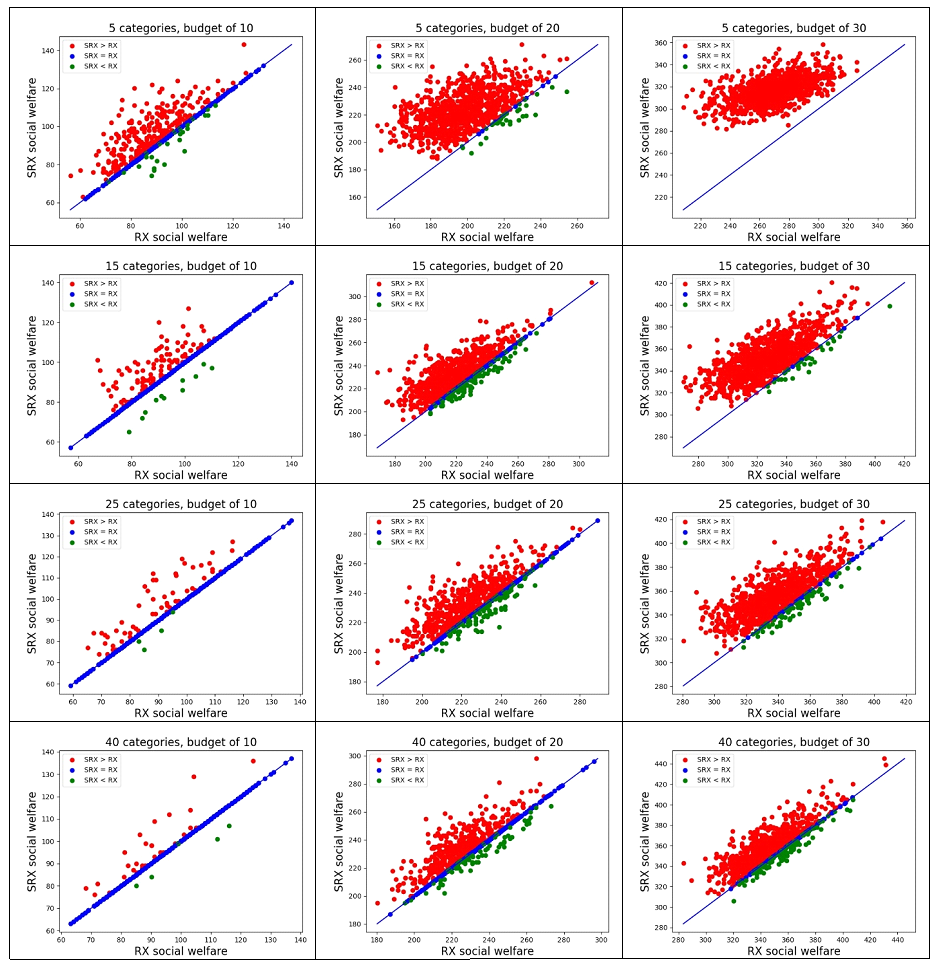
\includegraphics[width=14cm]{simulation/unit_scatters_no_prob.png}
\caption{SRX vs RX social welfare for different instance of Euclidean utilities simulations.
}\label{fig:scatter_all1}
\end{center}
\end{figure}

\begin{figure}[t]
\begin{center}
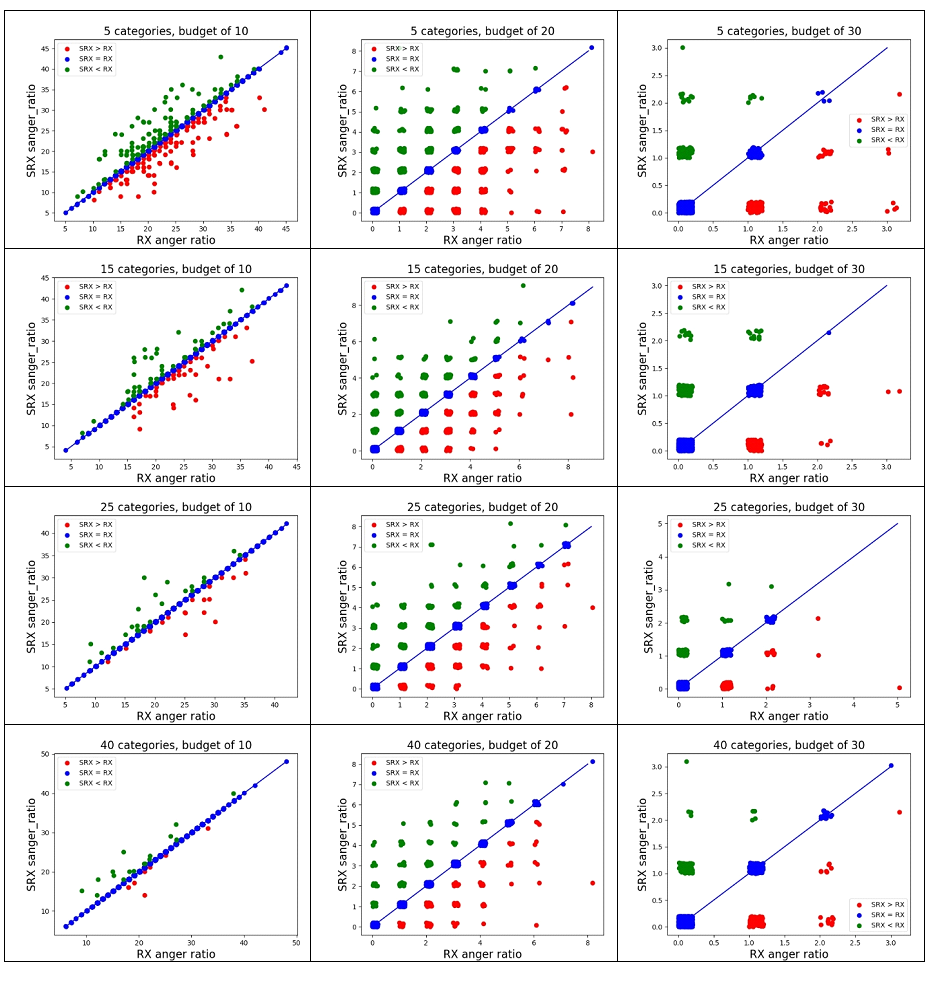
\includegraphics[width=14cm]{simulation/unit_scatters_ar.png}
\caption{SRX vs RX anger ratio for different instance of Euclidean utilities simulations.
}\label{fig:scatter_all_ar1}
\end{center}
\end{figure}

\begin{figure}[t]
\begin{center}
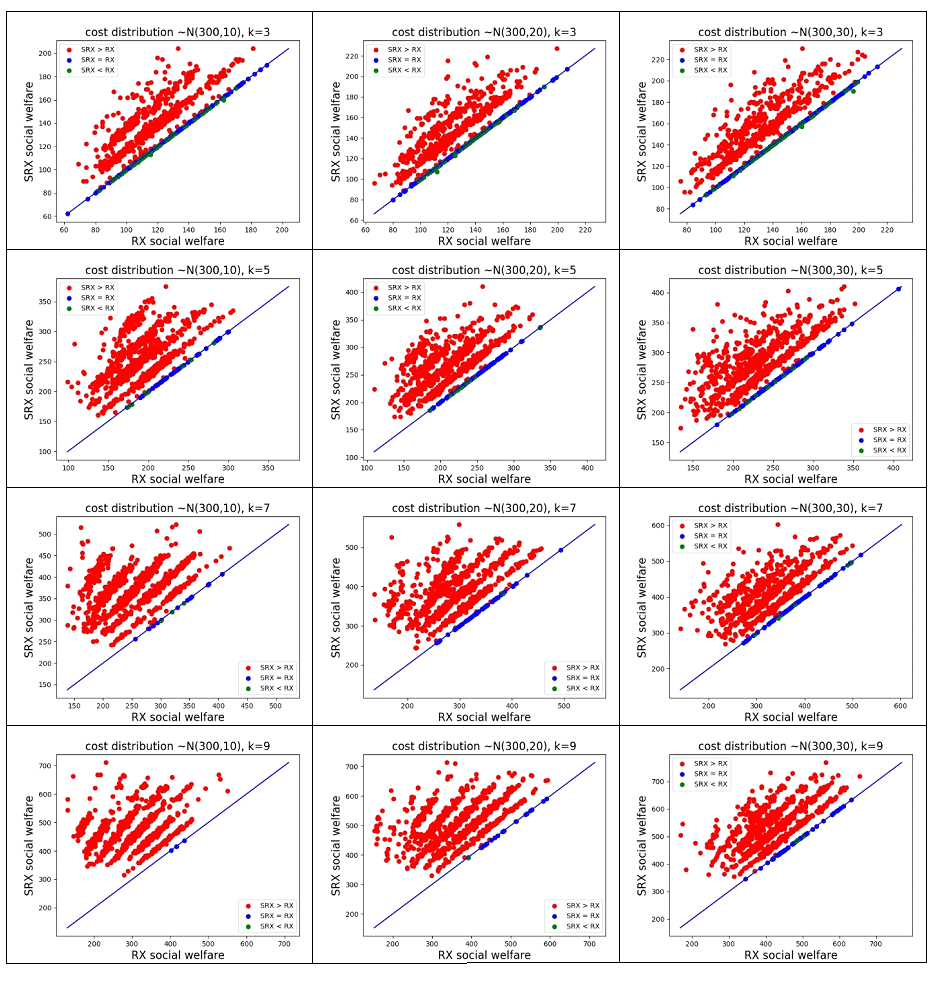
\includegraphics[width=14cm]{simulation/constant_scatters_no_prob.png}
\caption{SRX vs RX social welfare for different instance of global substitutes simulations.
}\label{fig:scatter_all2}
\end{center}
\end{figure}

\begin{figure}[t]
\begin{center}
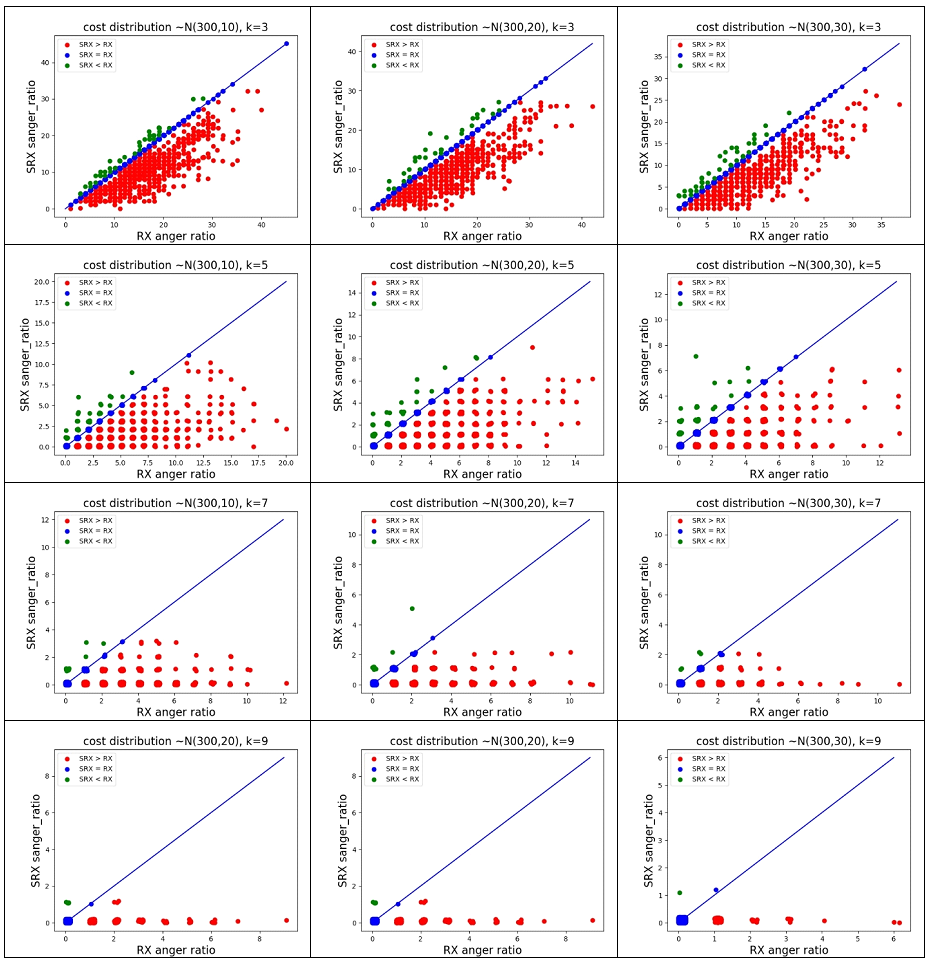
\includegraphics[width=14cm]{simulation/constant_scatters_ar.png}
\caption{SRX vs RX anger ratio for different instance of global substitutes simulations.
}\label{fig:scatter_all_ar2}
\end{center}
\end{figure}


\end{subappendices}

\end{document}
